\documentclass[10pt]{beamer}
\usepackage{uglixbeamer}
\title{Gestion des listes en \textsc{Python}}
\subtitle{Algorithmique}
\author{SIO1}
\begin{document}
\maketitle
\section{Opérations de base}

\begin{frame}[fragile]{Créer une liste}\pause
Pour créer une variable de type \pythoninline{list} on peut utiliser les commandes suivantes :\pause
\begin{itemize}
\item \pythoninline{L = list()} crée une liste vide;\pause
\item \pythoninline{L = []} fait la même chose;\pause
\item   \pythoninline{L = ['a', 7, True]} crée la liste composée de 3 éléments.\pause
\end{itemize}
Une liste peut contenir des éléments de plusieurs types mais en pratique on évite cela.
\end{frame}

\begin{frame}[fragile]{Modifier un élément}\pause
Le type \pythoninline{list} est \alert{mutable}, cela veut dire qu'on peut changer les éléments d'une liste sans changer la liste en elle-même (on précisera pourquoi et comment plus tard dans ce document).\\\pause

Pour changer le deuxième élément d'une liste \pythoninline{L} qui vaut \pythoninline{[2, 3, 4, 1]} on écrira\pause \begin{center}
\pythoninline{L[1] = 10}
\end{center}\pause
et la liste aura la valeur \pythoninline{[2, 10, 4, 1]}.
\end{frame}
\begin{frame}[fragile]{Ajouter un élément à une liste}\pause

\pythoninline{L.append(4)} ajoute la valeur 4 à la fin de la liste \pythoninline{L}.\\\pause

\pythoninline{L = L + [4]} a le même effet : on crée une \og mini-liste\fg{} \pythoninline{[4]}, on concatène les 2 listes et on remet le résultat dans \pythoninline{L}.\\\pause

En pratique la première méthode est la plus simple et aussi la plus rapide.\\
\end{frame}
\begin{frame}[fragile]{Retirer un élément à une position donnée}\pause
Si une liste \pythoninline{L} a pour valeur \pythoninline{[3 ,7, 1]} et qu'on veut supprimer son deuxième élément alors on écrit\pause \begin{center}
\pythoninline{del L[1]}
\end{center}\pause
Ensuite, \pythoninline{L} aura la valeur \pythoninline{[3,1]}.
\end{frame}
\begin{frame}[fragile]{Retirer une valeur précise}\pause
Pour retirer une valeur \alert{qui appartient à une liste} on procède ainsi :\\\pause

Si \pythoninline{L} a la valeur \pythoninline{[1, 2, 5, 4, 2, 3]} alors l'instruction\pause \begin{center}
\pythoninline{L.remove(2)}
\end{center}\pause
Supprime la \alert{première occurrence} de \pythoninline{2} dans \pythoninline{L}.\\\pause
Ainsi \pythoninline{L} a la valeur \pythoninline{[1, 5, 4, 2, 3]}.
\end{frame}

\begin{frame}[fragile]{Ajouter des listes}\pause
On peut procéder de 2 manières : \pause
\begin{itemize}
\item \pythoninline{L.extend(M)} ajoute les éléments de la liste \pythoninline{M} à la fin de \pythoninline{L};\pause
\item \pythoninline{L = L + M} crée une liste avec les éléments de \pythoninline{L} puis ceux de \pythoninline{L} et replace le résultat dans \pythoninline{L}.\pause
\end{itemize}
En pratique la première méthode est plus rapide.\\
\end{frame}

\begin{frame}{Divers}\pause
\pythoninline{L.sort()} trie la liste dans l'ordre croissant.\\\pause

\pythoninline{L.reverse()} met les éléments dans l'ordre inverse.\pause
\end{frame}
\section{Manipulations}
\begin{frame}[fragile]{Copier une liste (mauvaise méthode)}\pause
\begin{minted}{python}
L = [3, 5, 2]
M = L
M[0] = 2
print(M) # Affiche [2, 5, 2]
print(L) # Affiche [2, 5, 2] aussi. Aïe !
\end{minted}
\pause
Ce comportement \og étrange\fg{} vient du fait que le type \pythoninline{list} est mutable. Nous allons expliquer cela plus tard dans ce document.
\end{frame}

\begin{frame}[fragile]{Copier une liste (bonne méthode)}\pause
\begin{minted}{python}
L = [3, 5, 2]
M = L[:] # on copie tous les éléments de L dans M
M[0] = 2
print(M) # Affiche [2, 5, 2]
print(L) # Affiche [3, 5, 2] aussi. Ouf !
\end{minted}
\end{frame}
\section{Mutabilité}
\begin{frame}{variables de type non-mutable}\pause

	\only<1>{Les variables de type \mintinline{python}{int} sont non-mutables.}
	\only<2>{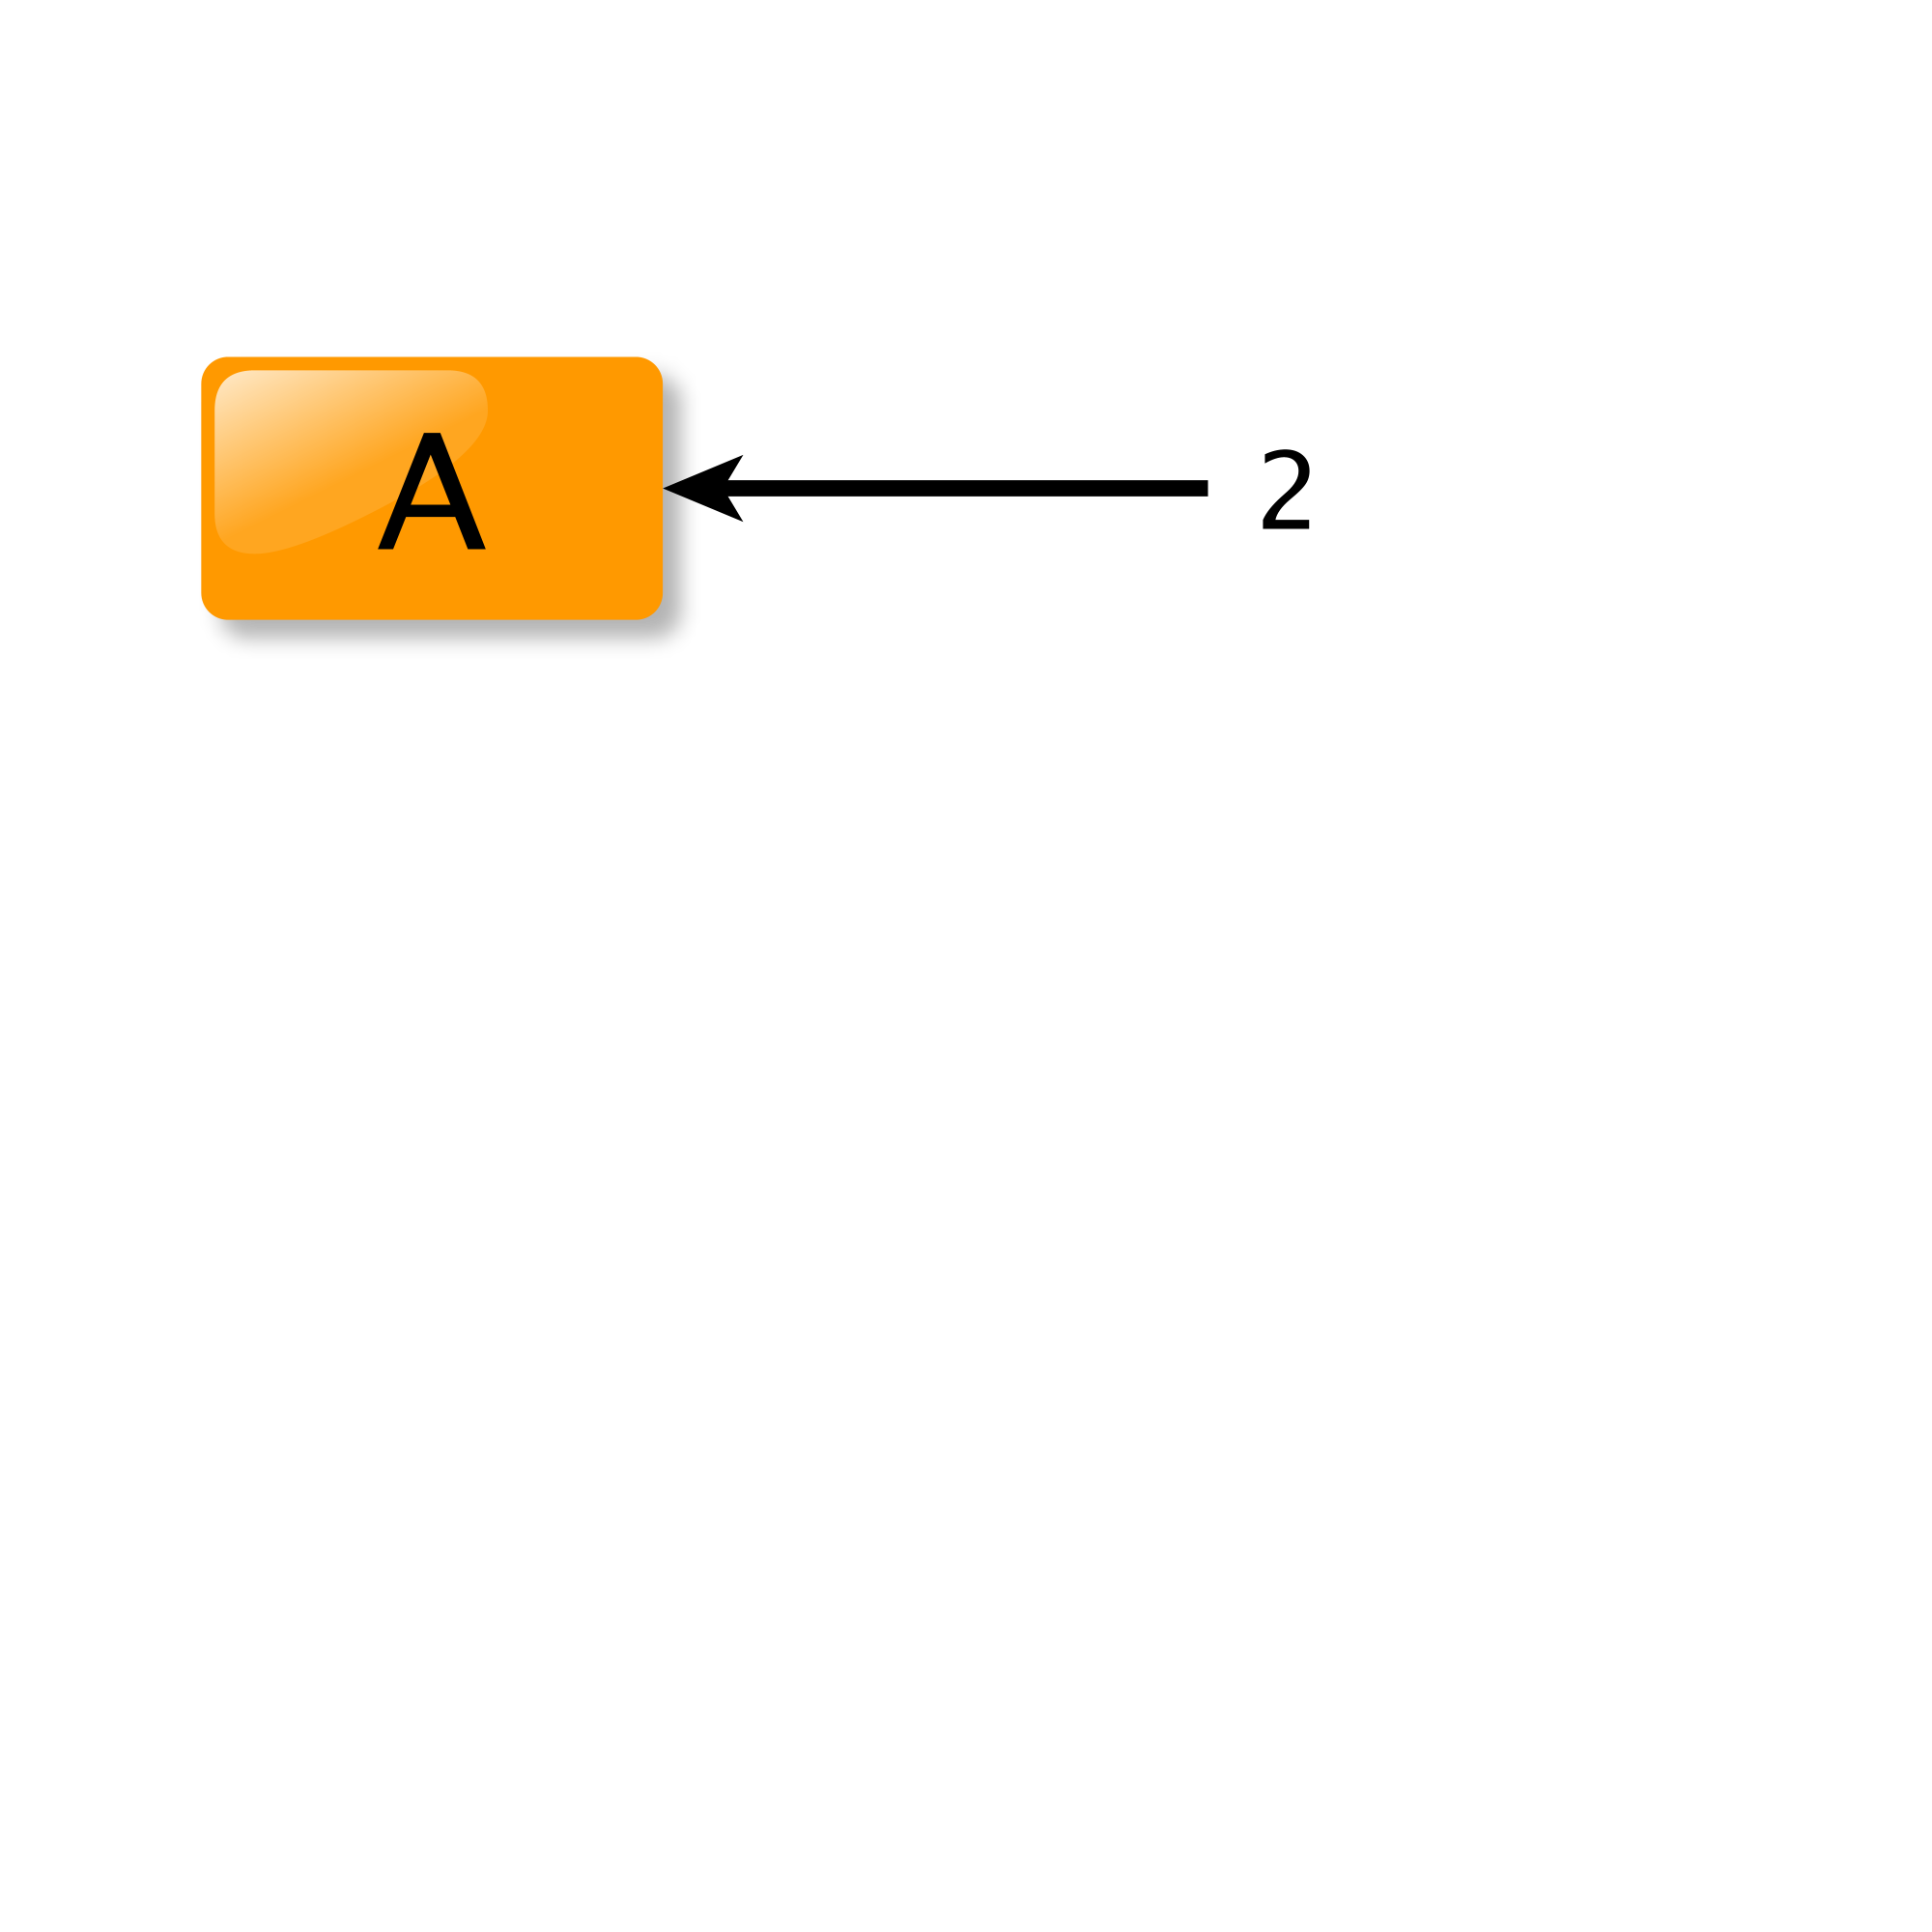
\includegraphics[width=6cm]{img/v0}\\ On affecte 2 à A.}
	\only<3>{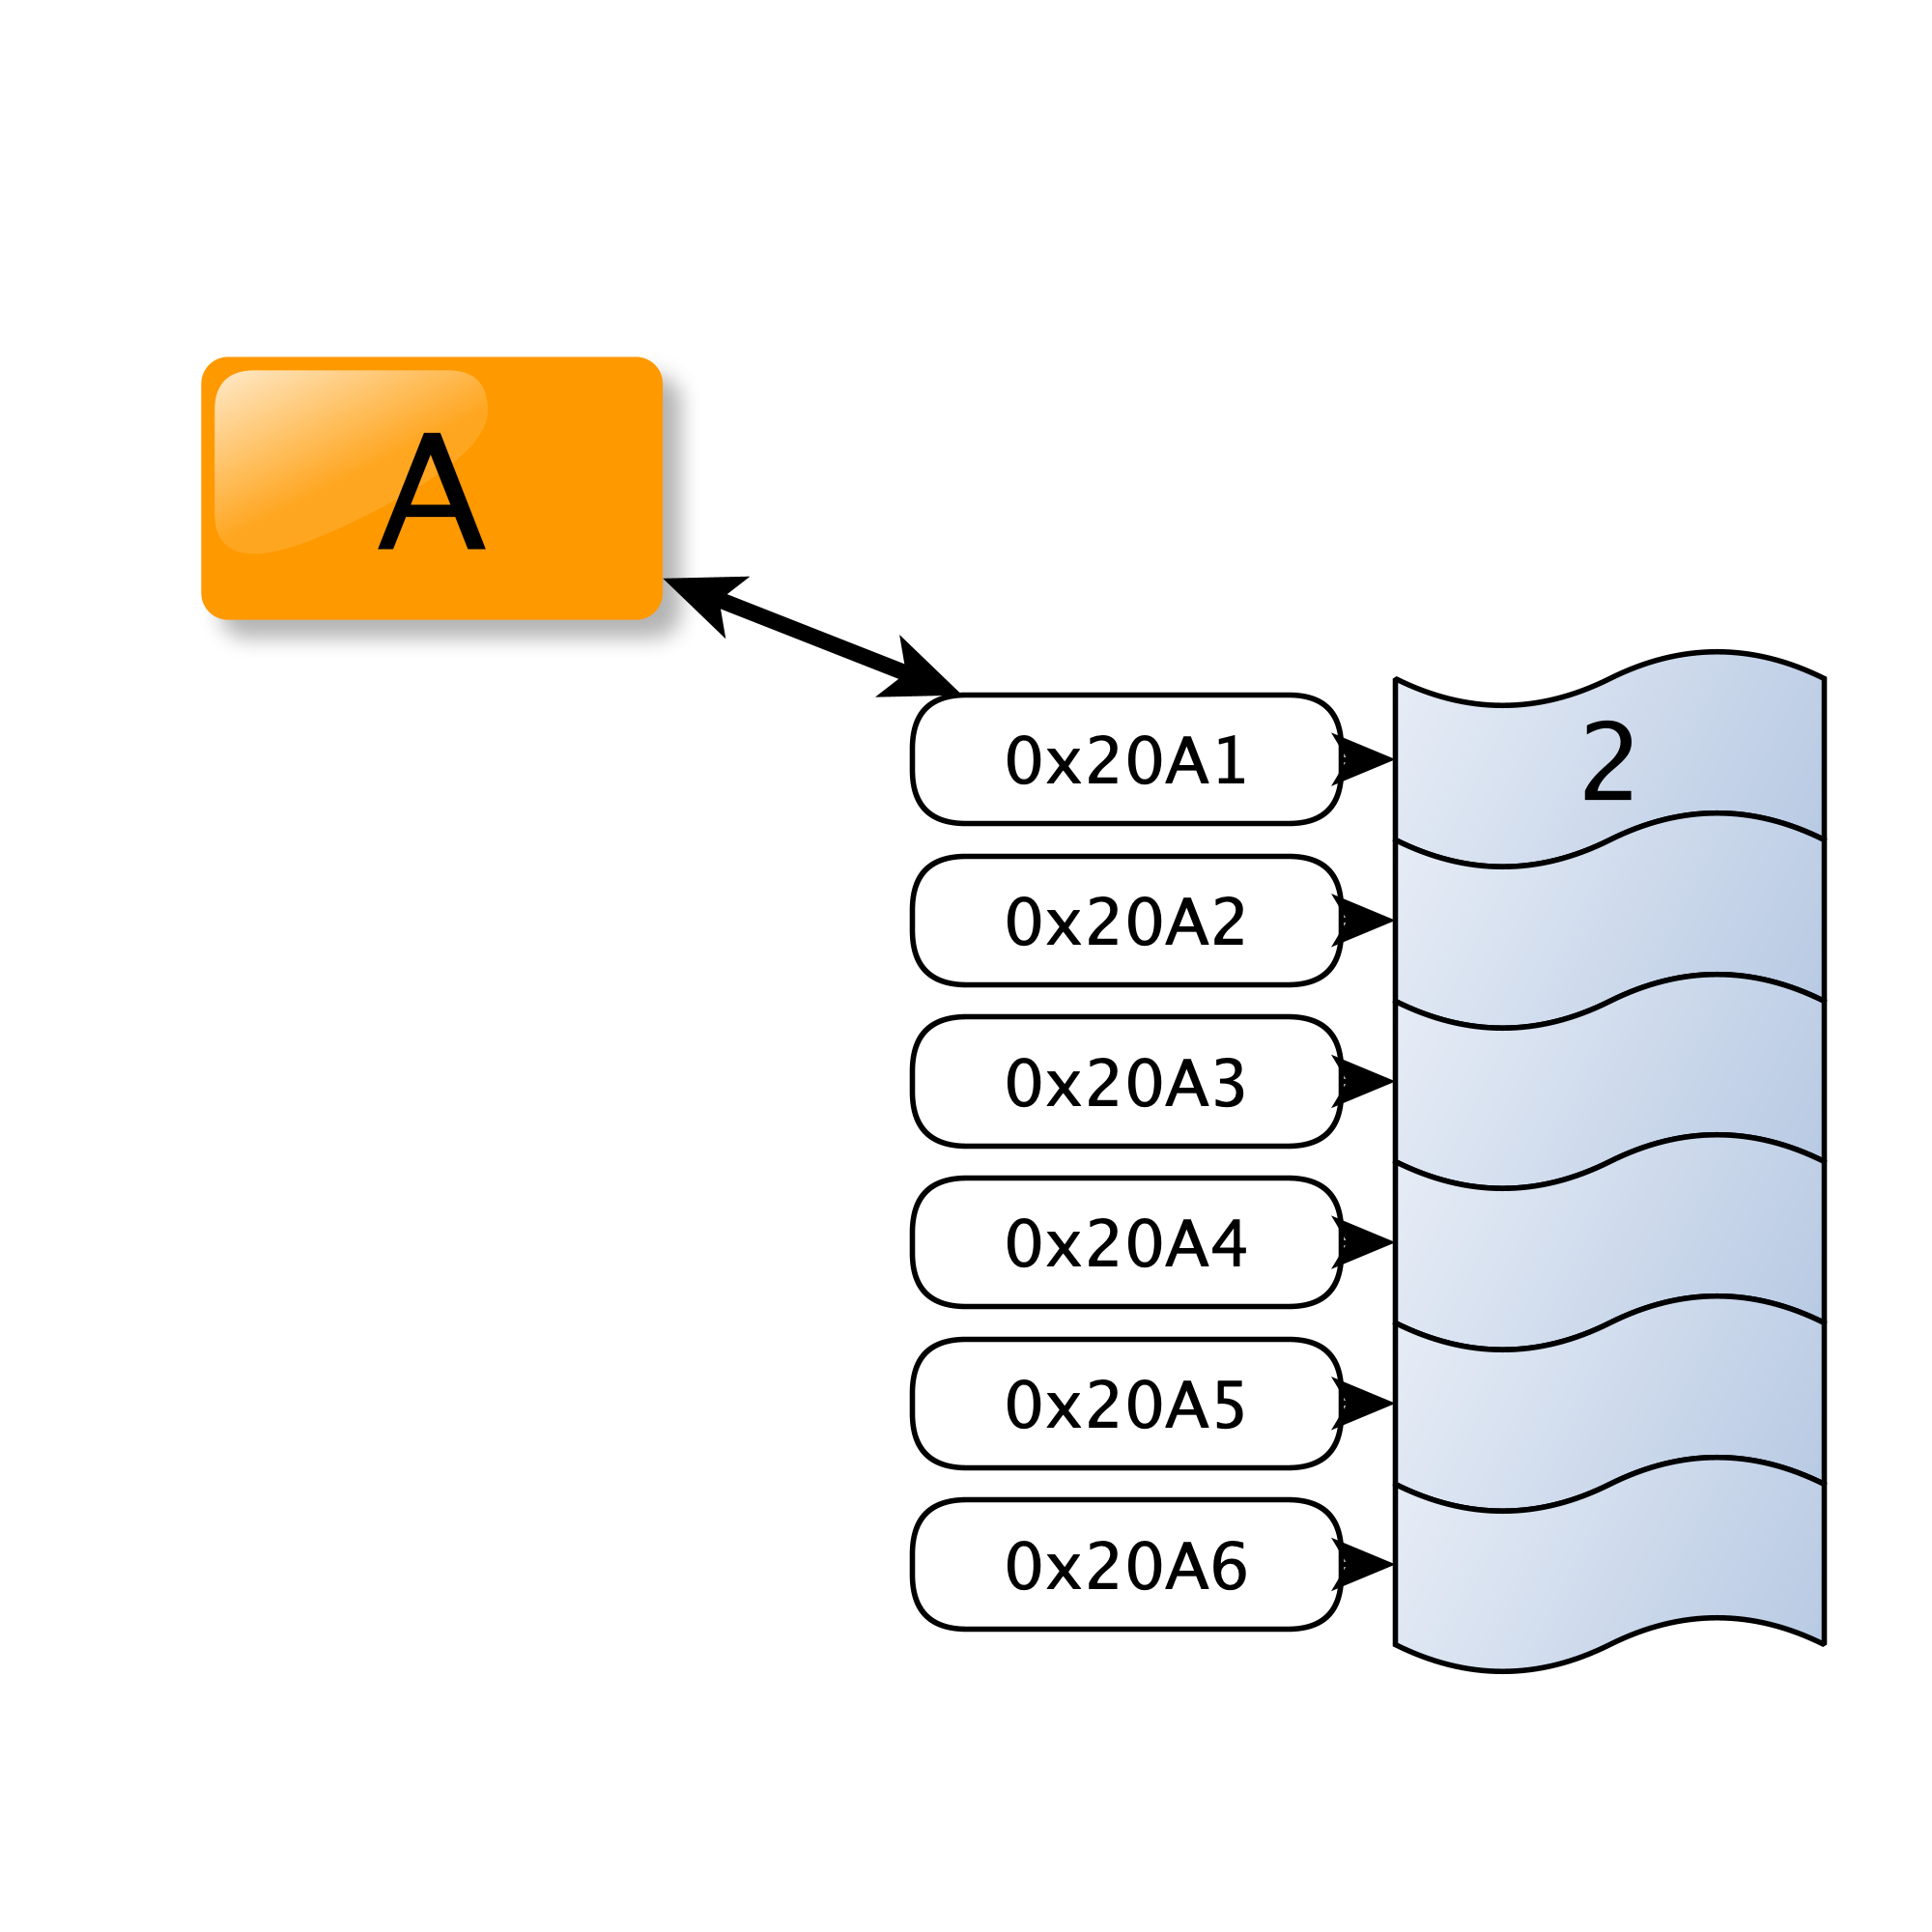
\includegraphics[width=6cm]{img/v1}\\ Une adresse mémoire est réservée. }
	\only<4>{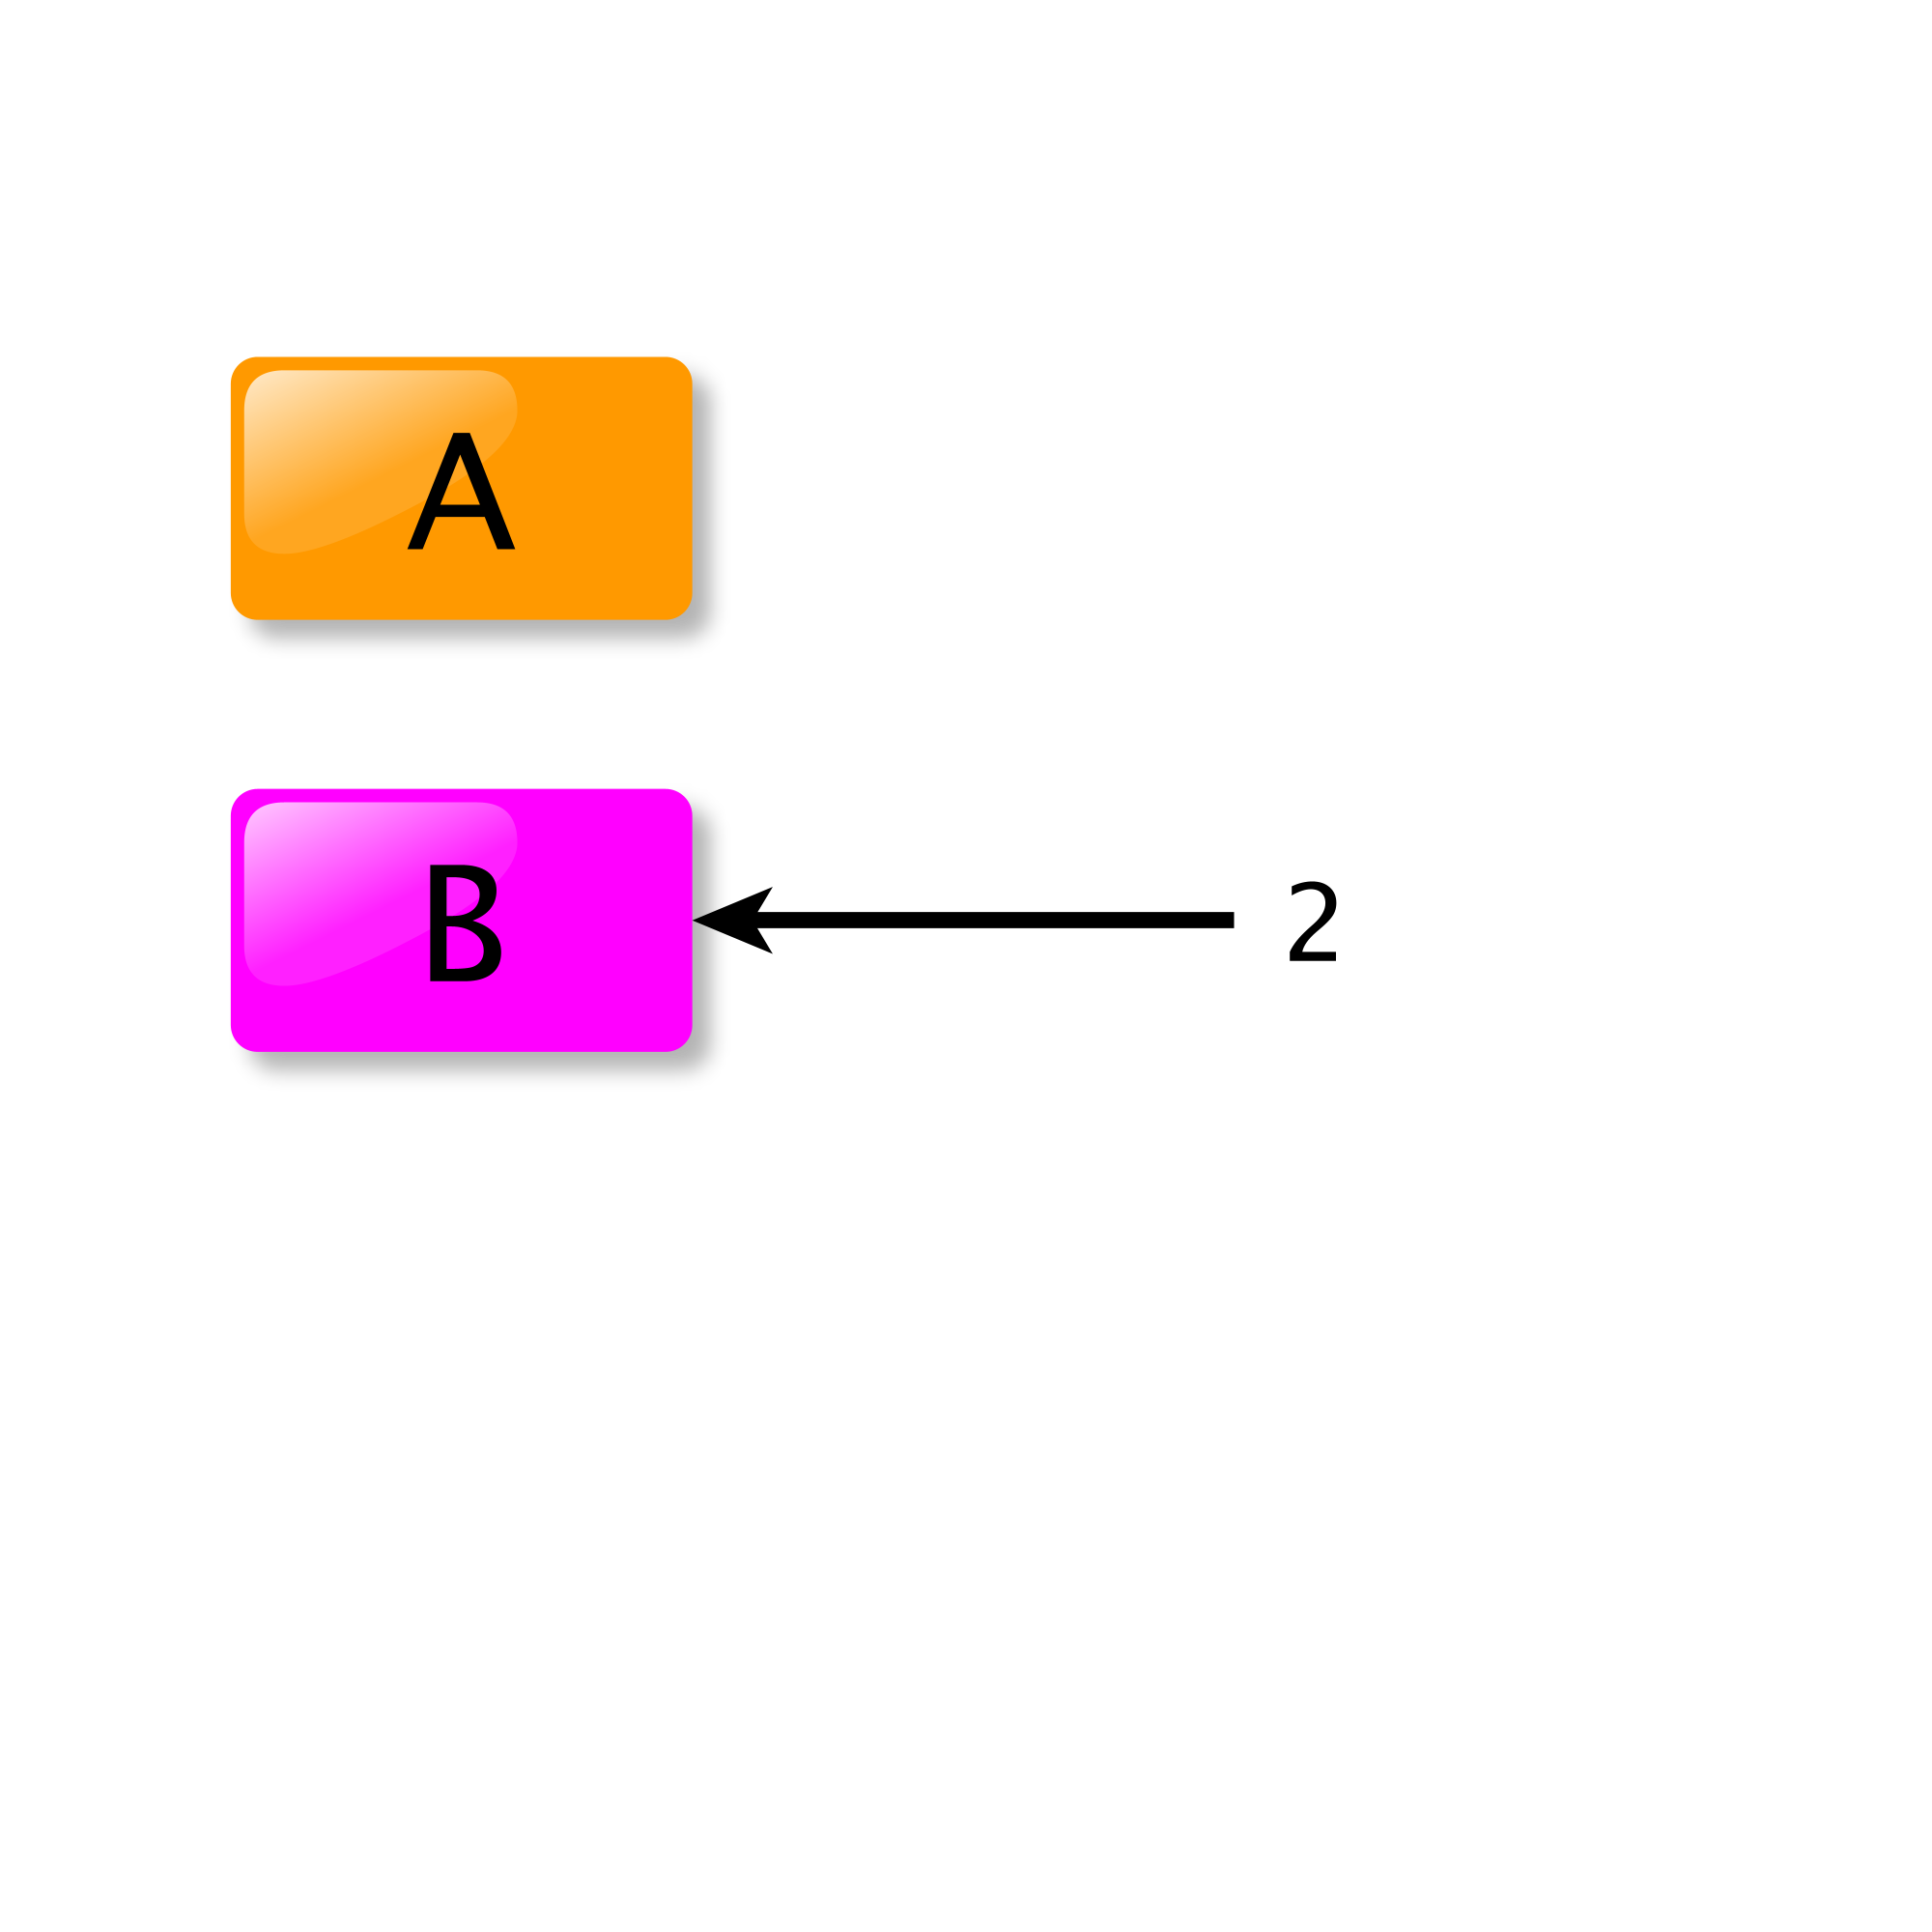
\includegraphics[width=6cm]{img/v2}\\ On affecte 2 à B.}
	\only<5>{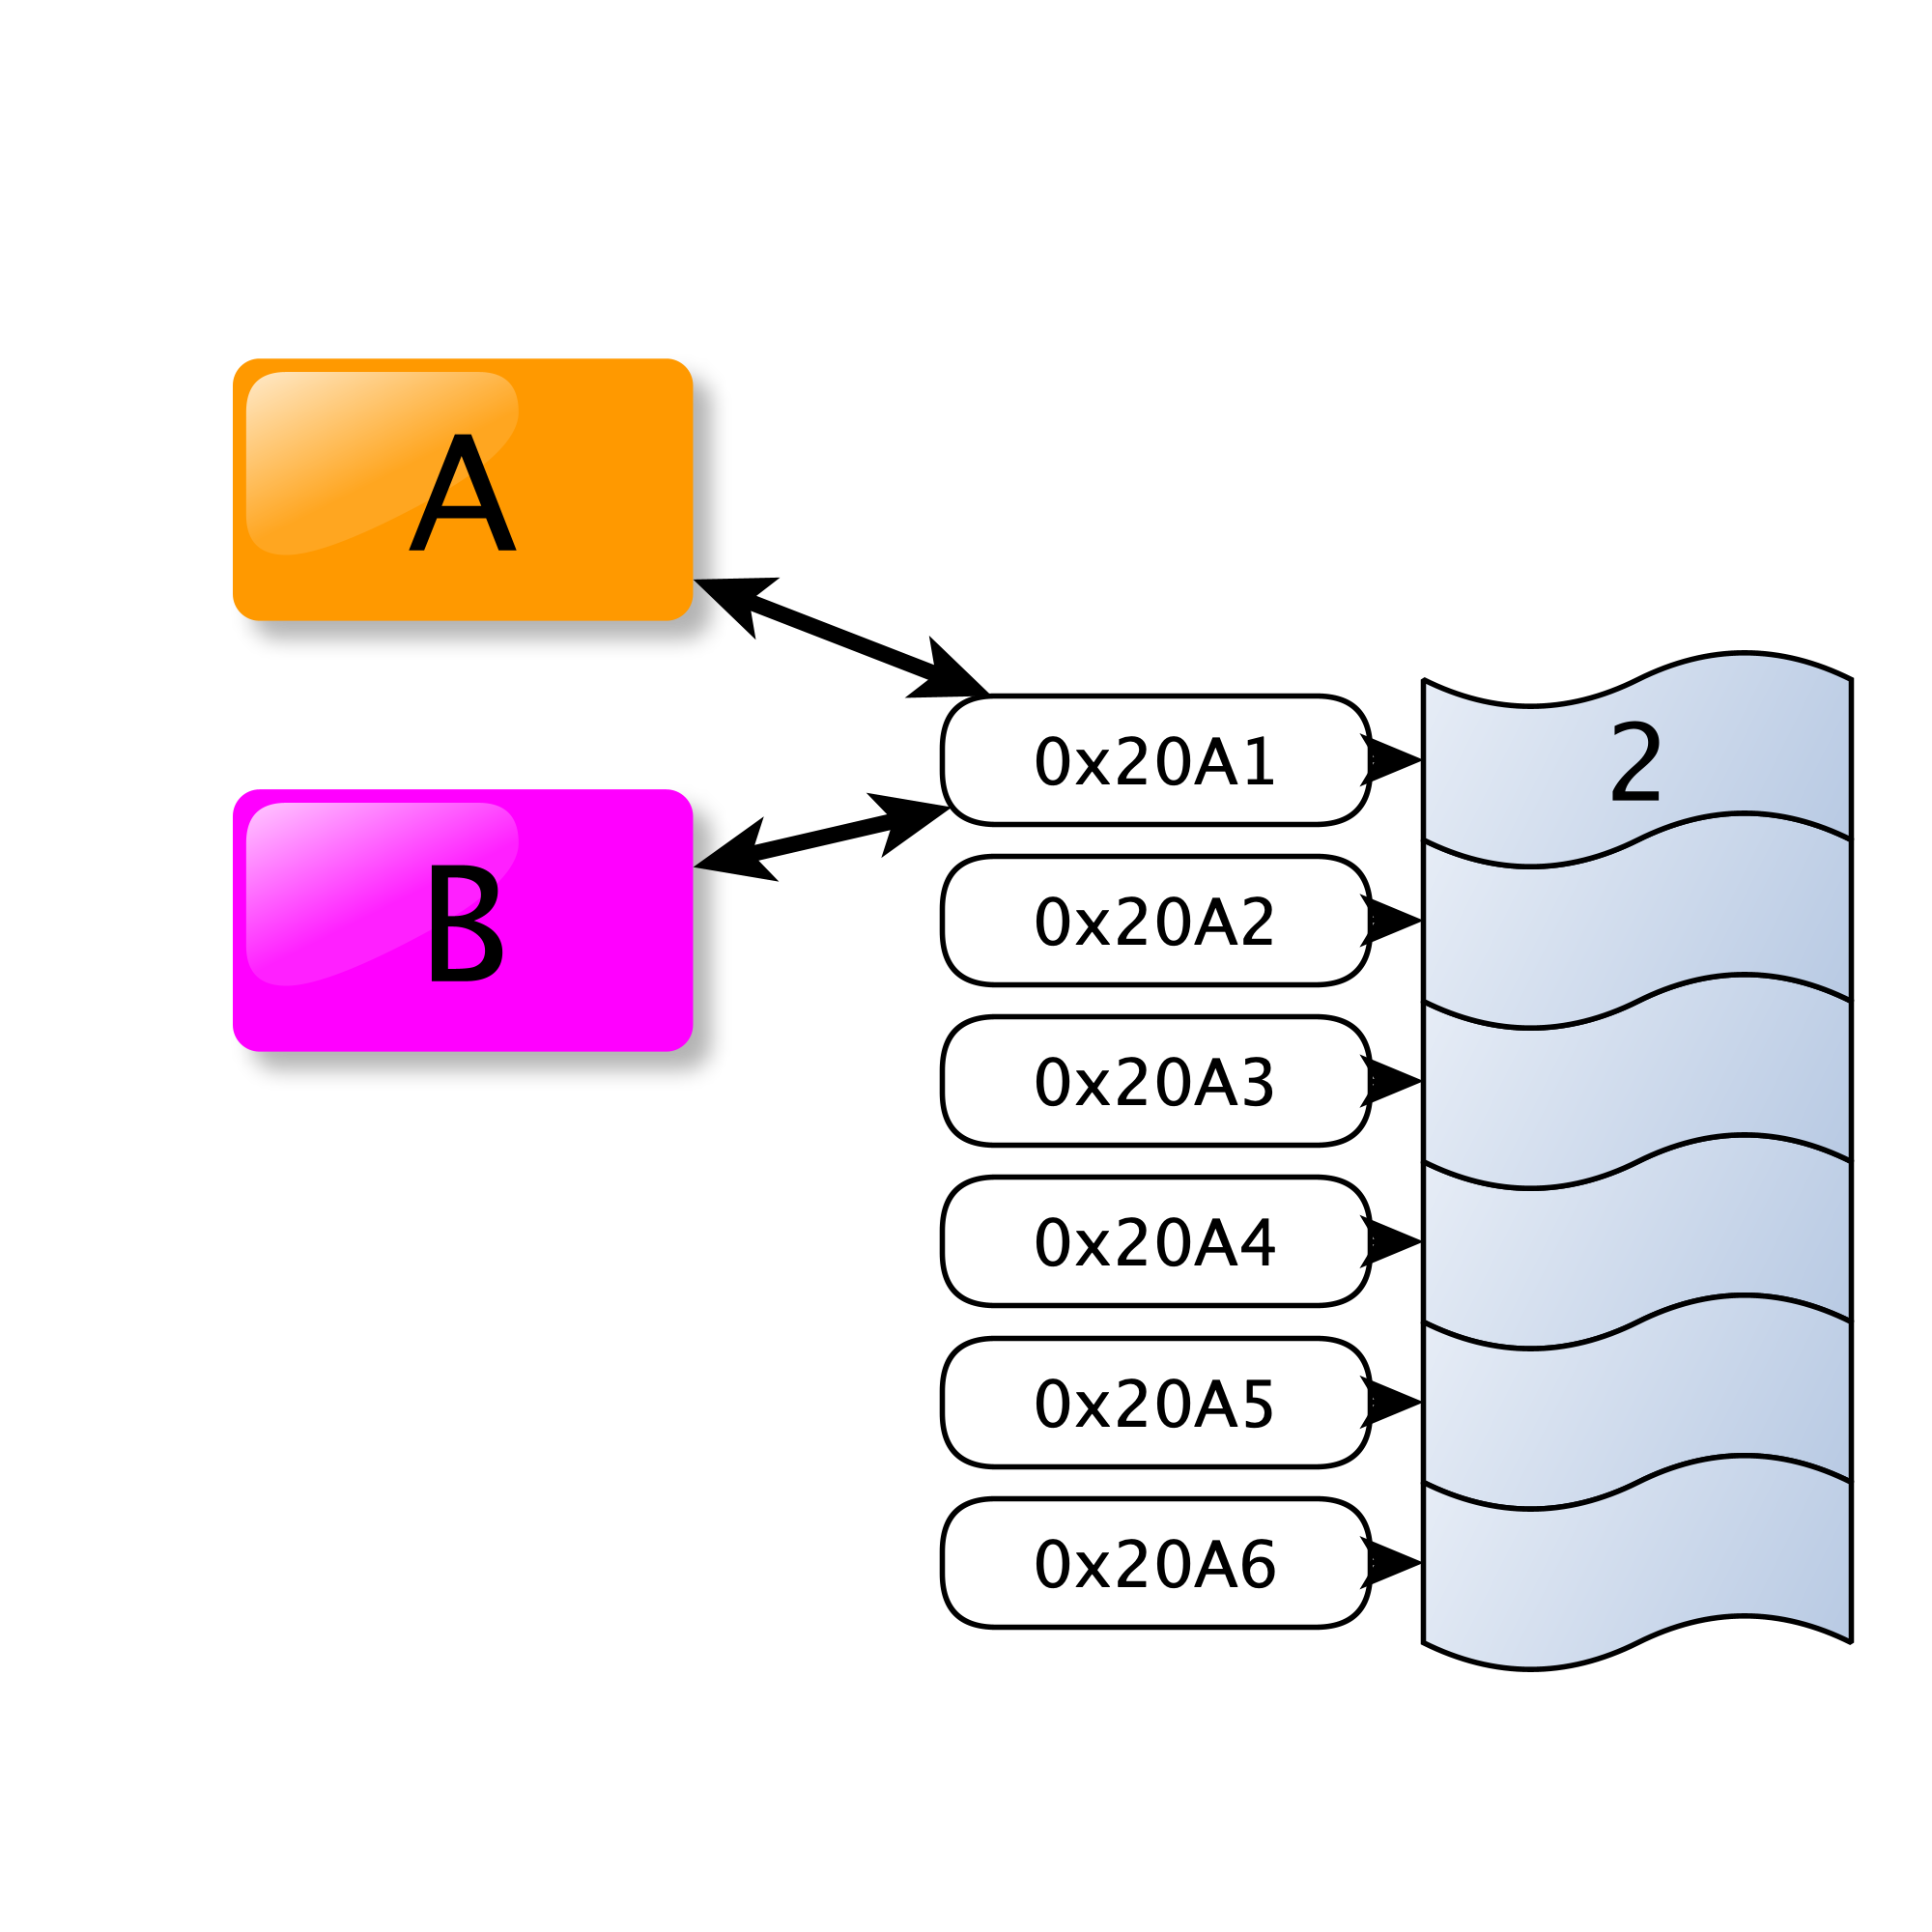
\includegraphics[width=6cm]{img/v3}\\ A et B pointent sur la même adresse.}
	\only<6>{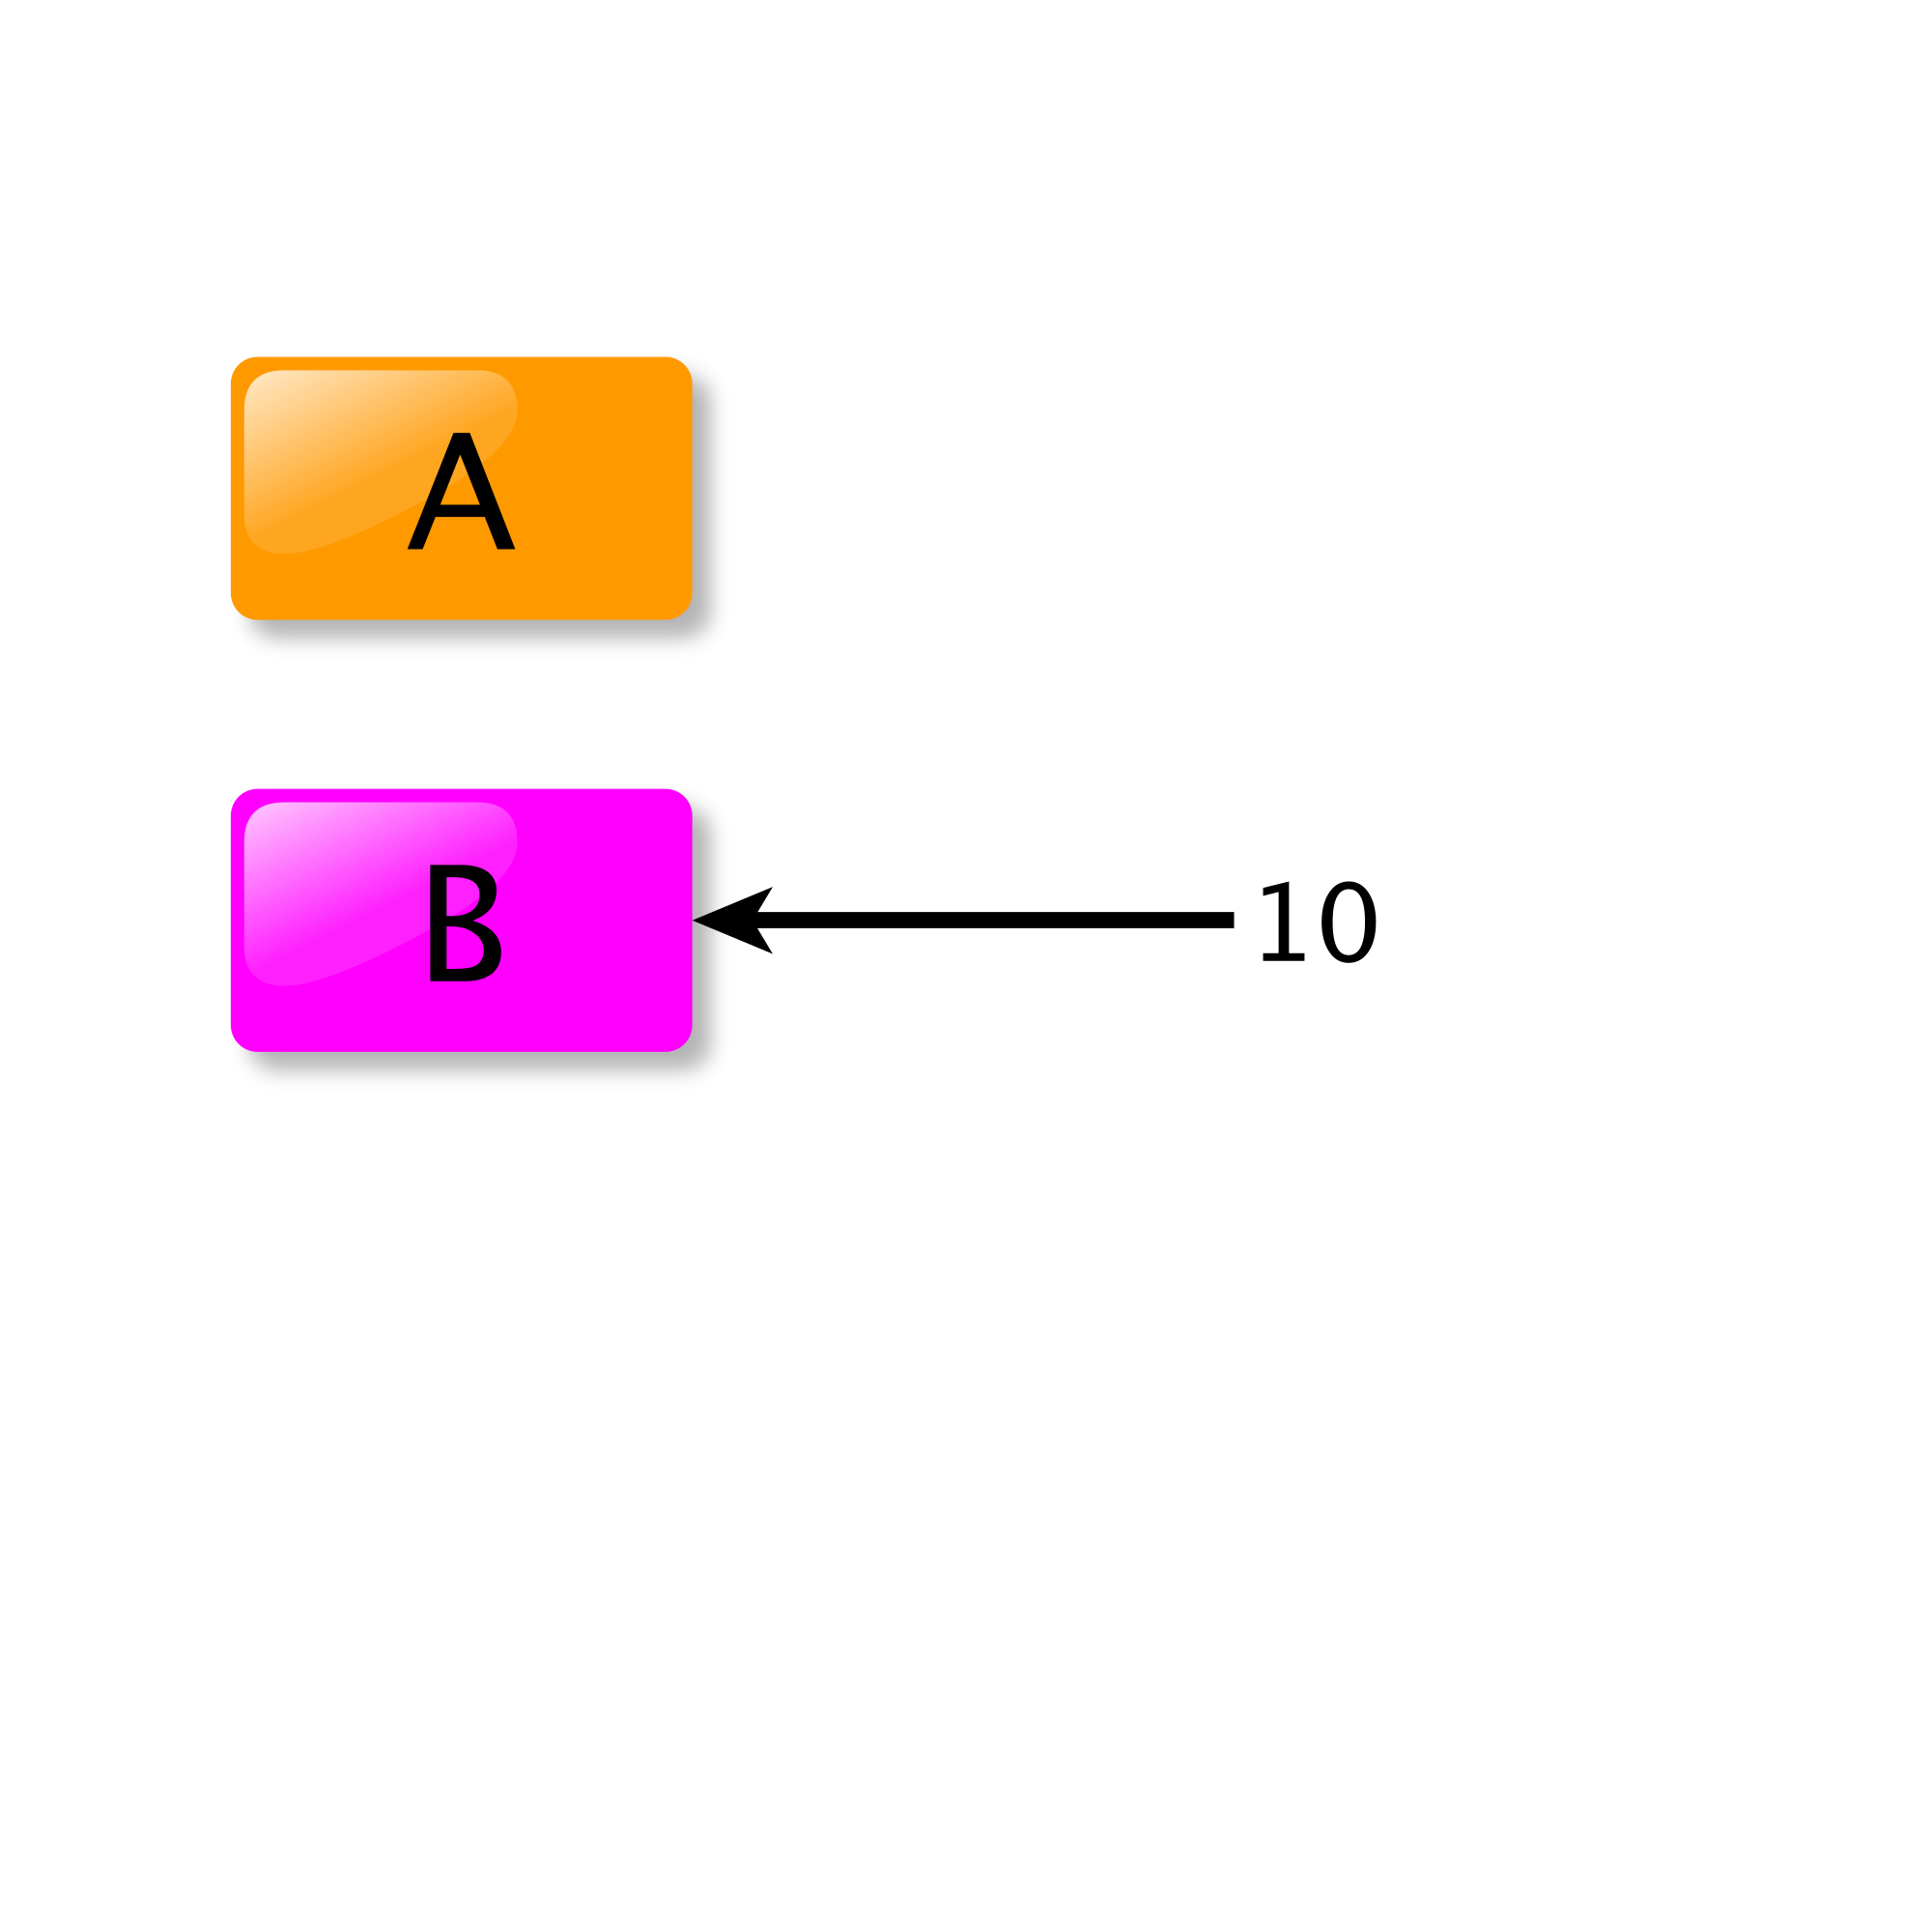
\includegraphics[width=6cm]{img/v4}\\ On change la valeur de B.}
	\only<7>{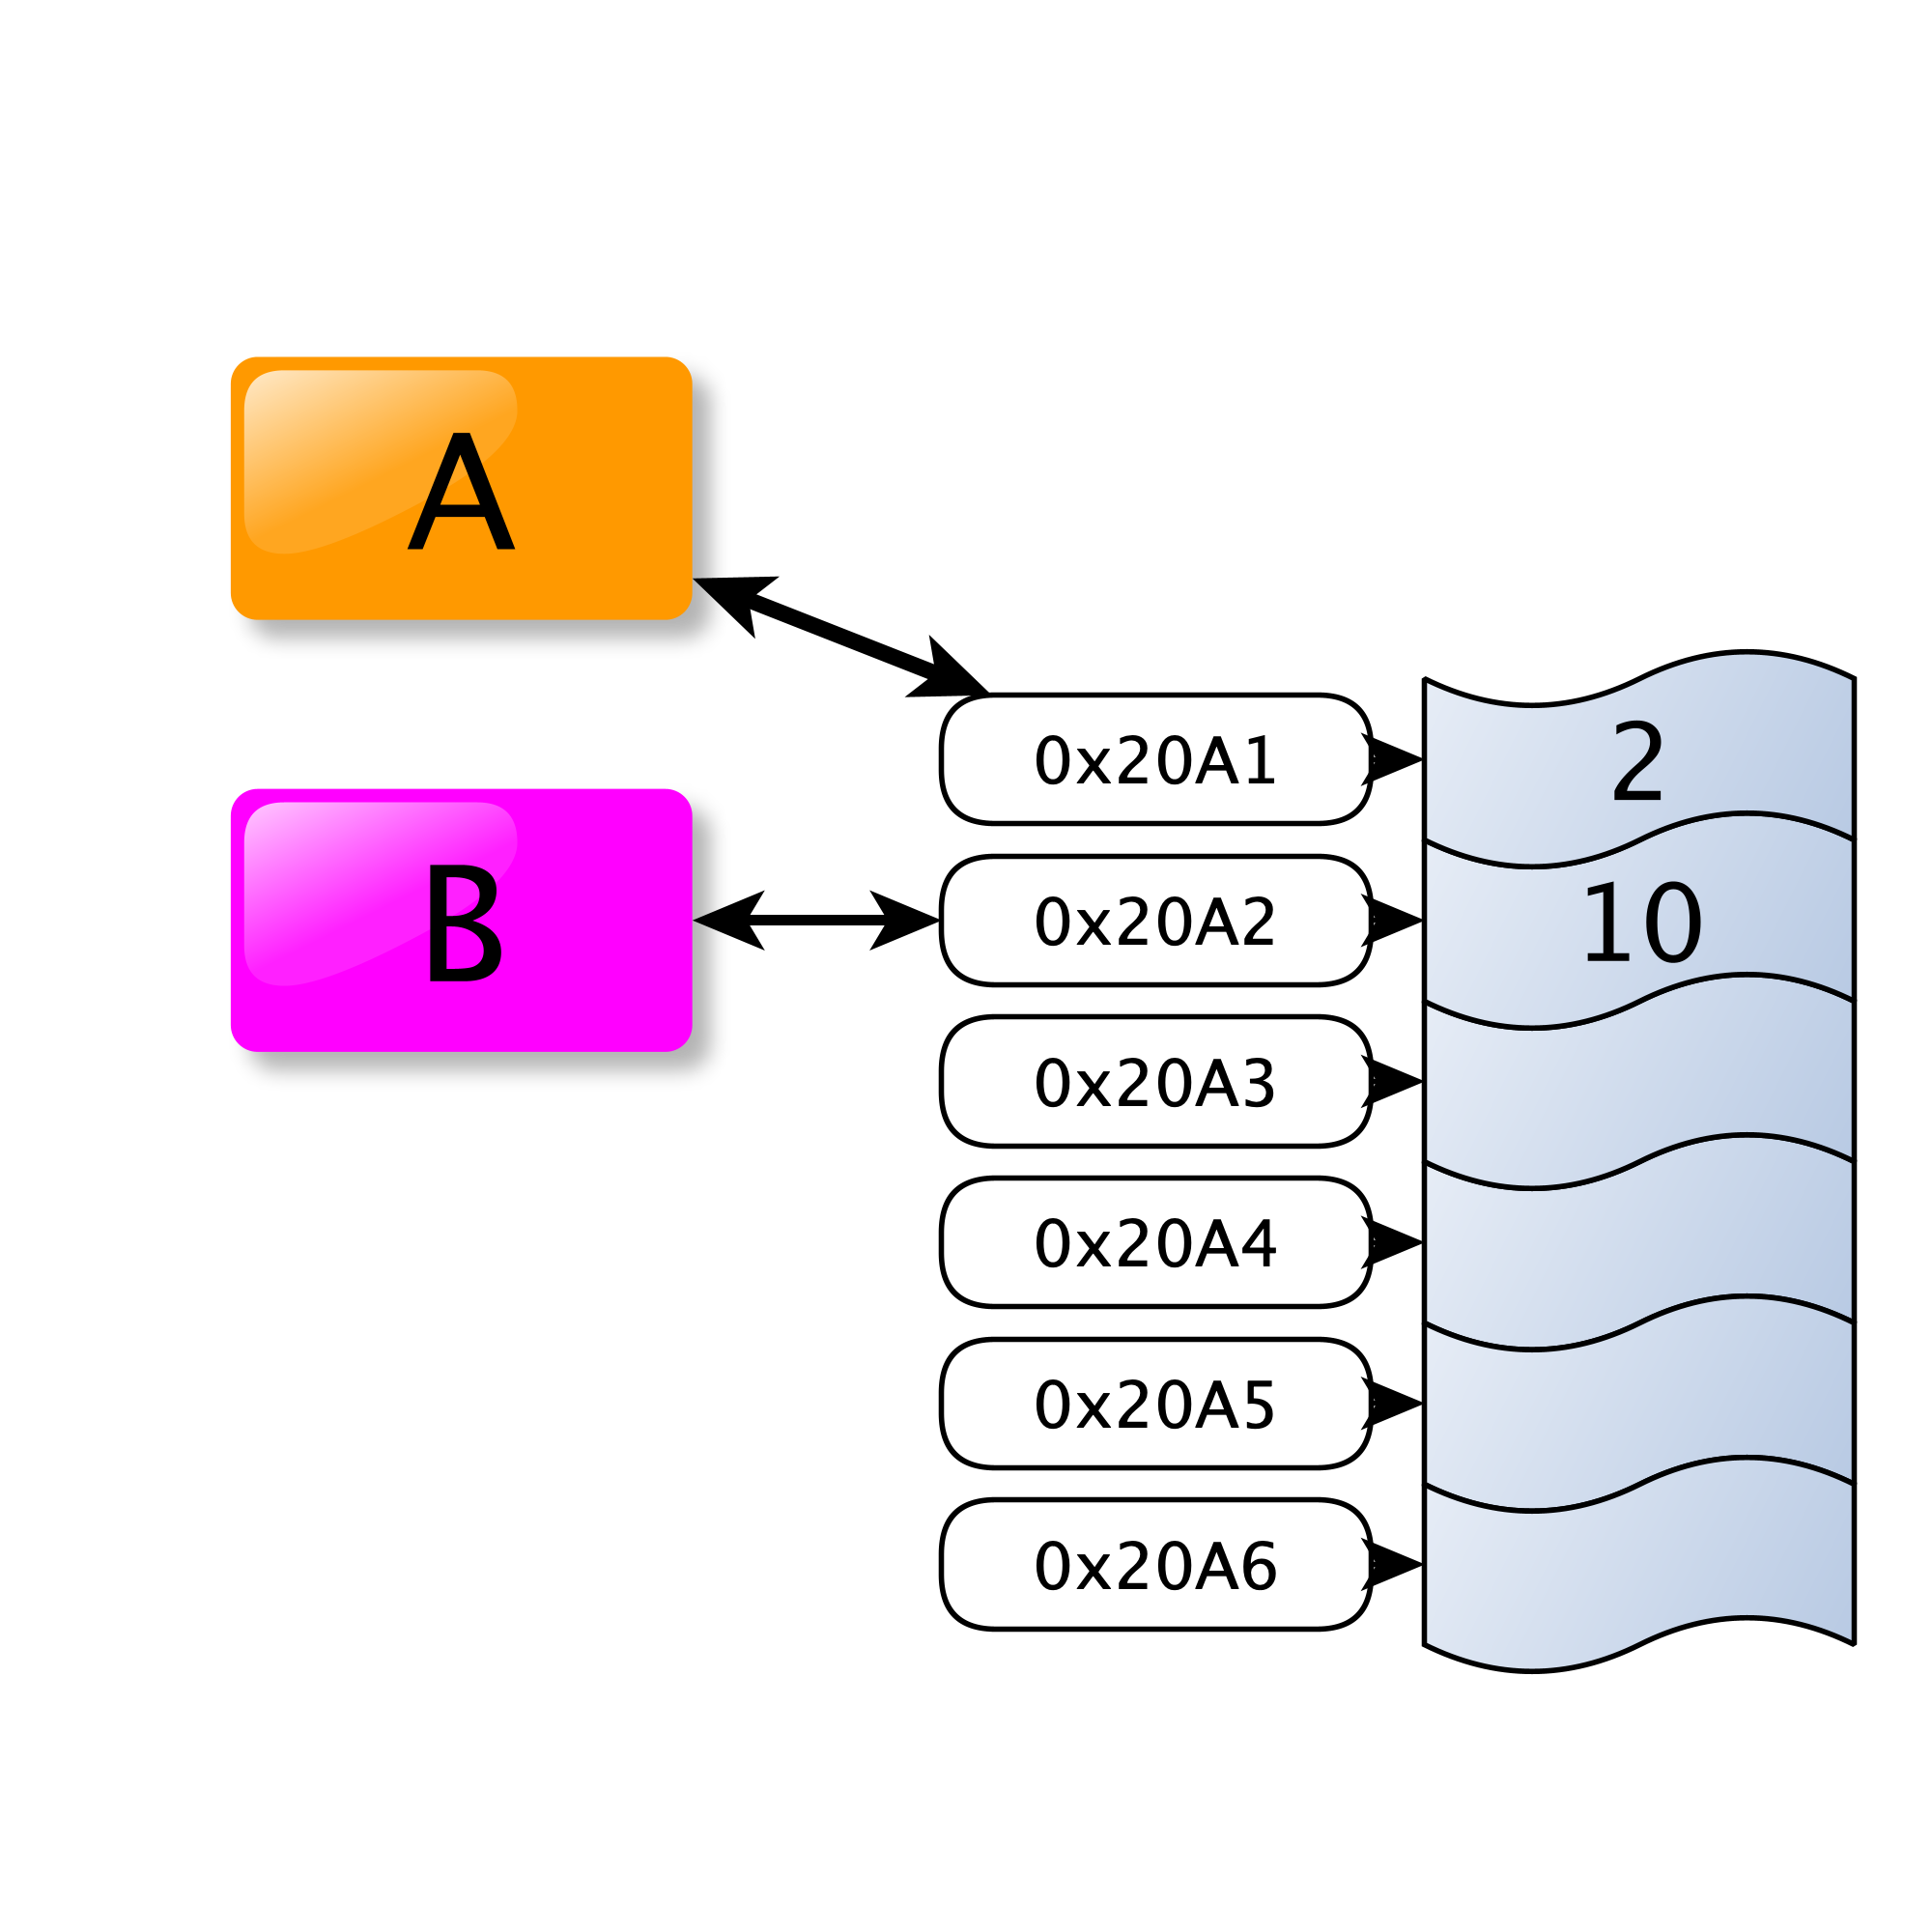
\includegraphics[width=6cm]{img/v5}\\ B pointe sur une autre adresse.}
\end{frame}

\begin{frame}{variables de type mutable}\pause
	\only<1>{Les variables de type \mintinline{python}{list} sont \alert{mutables}.}
	\only<2>{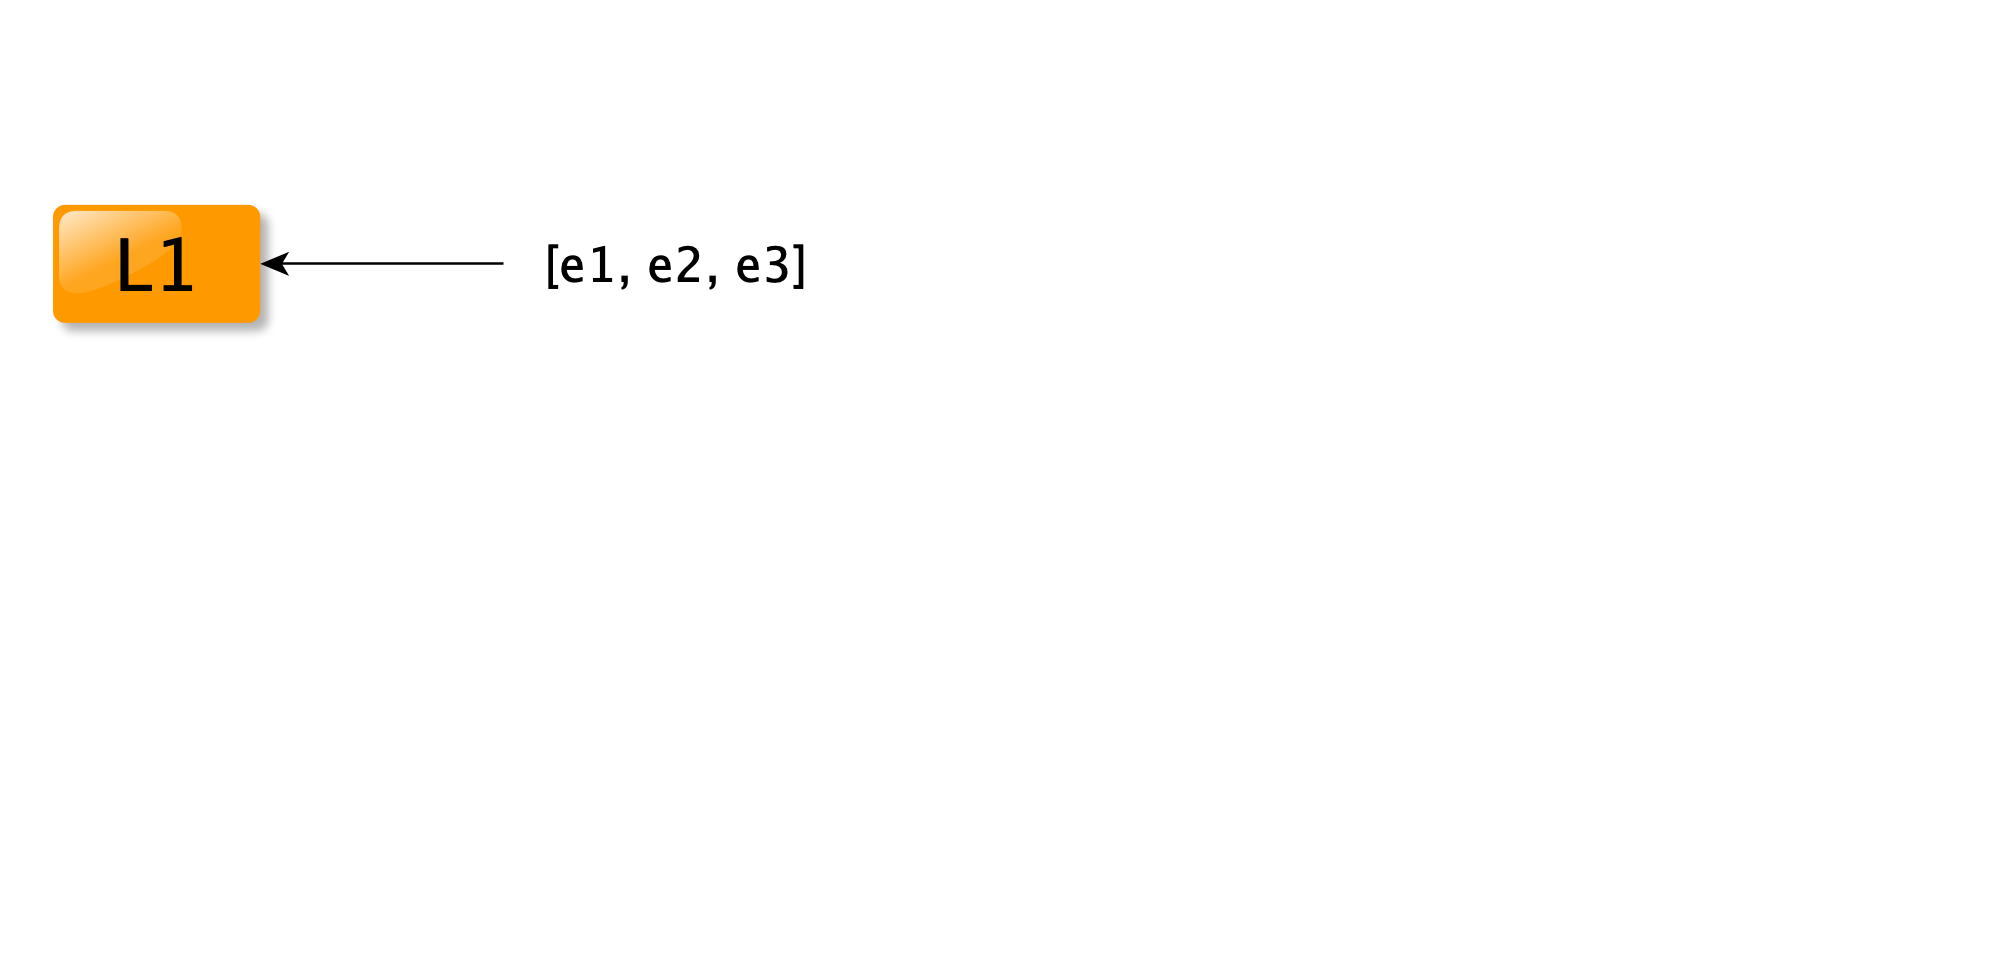
\includegraphics[width=10cm]{img/L0}\\ On affecte [e1, e2, e3] à L1.}
	\only<3>{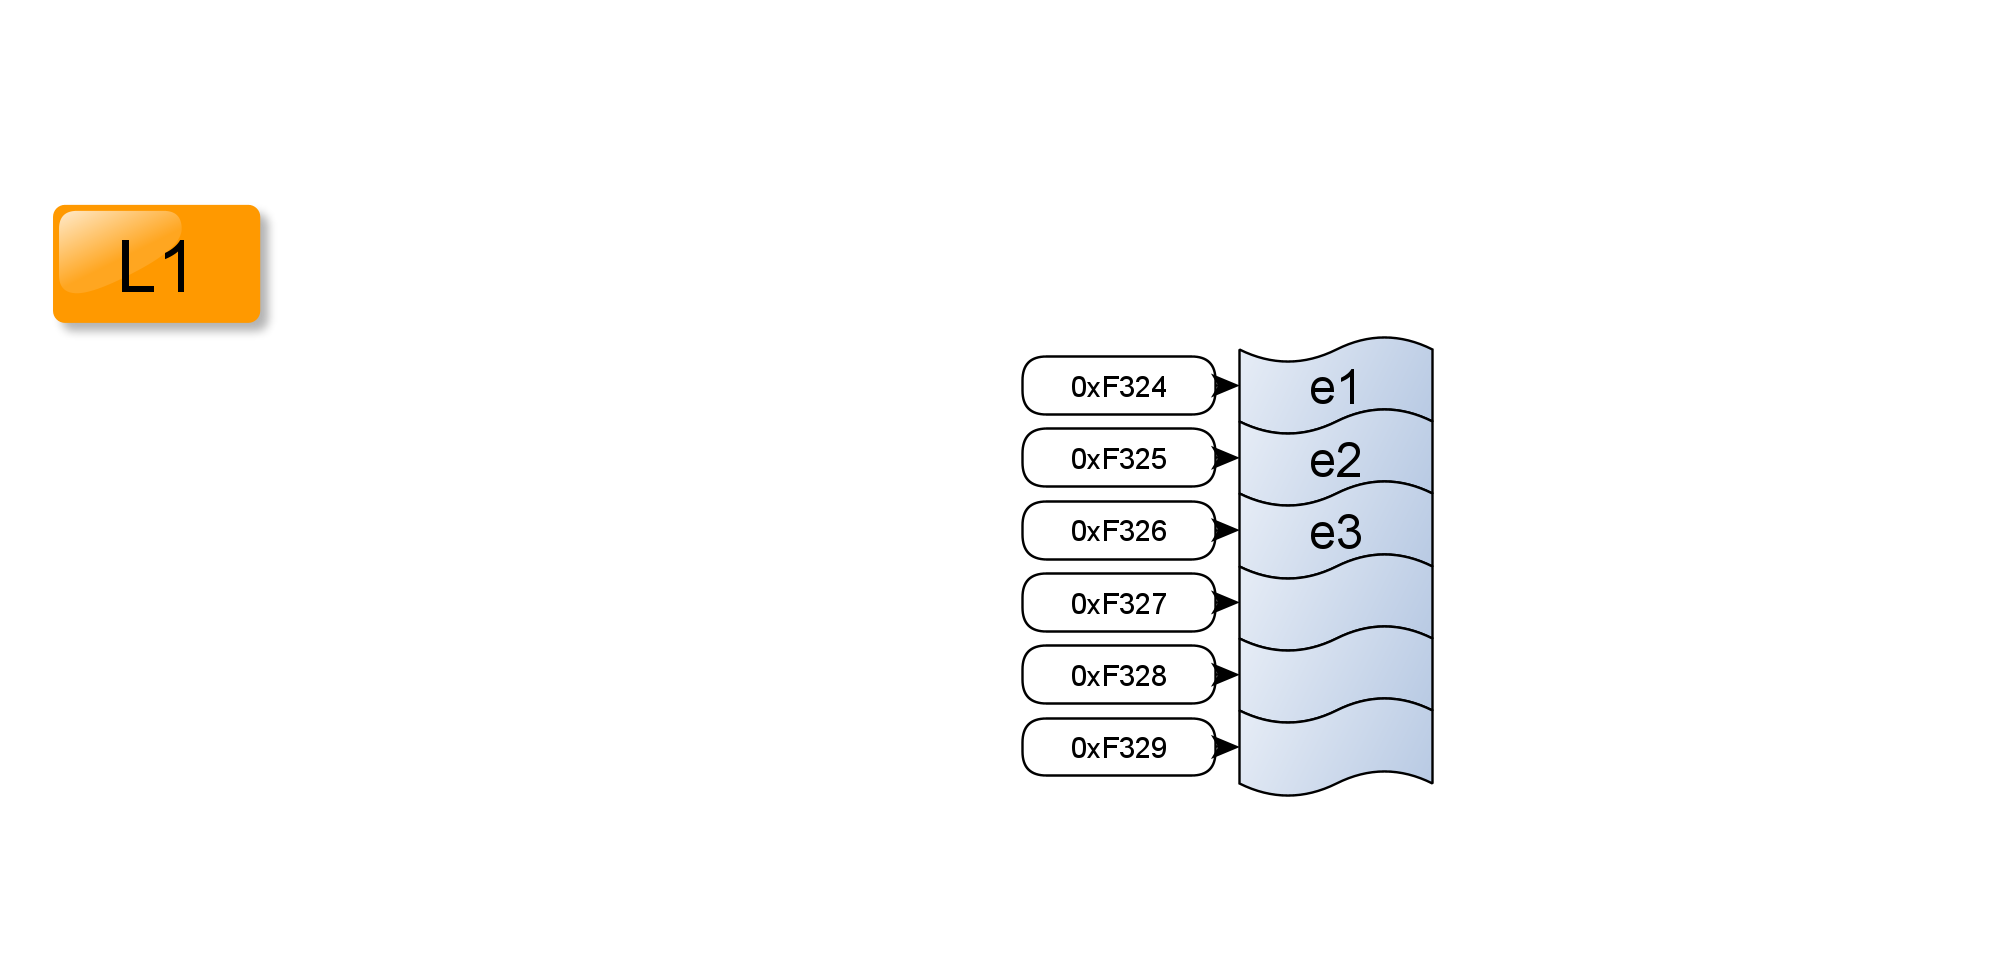
\includegraphics[width=10cm]{img/L1}\\ Les éléments sont mis en mémoire. }
	\only<4>{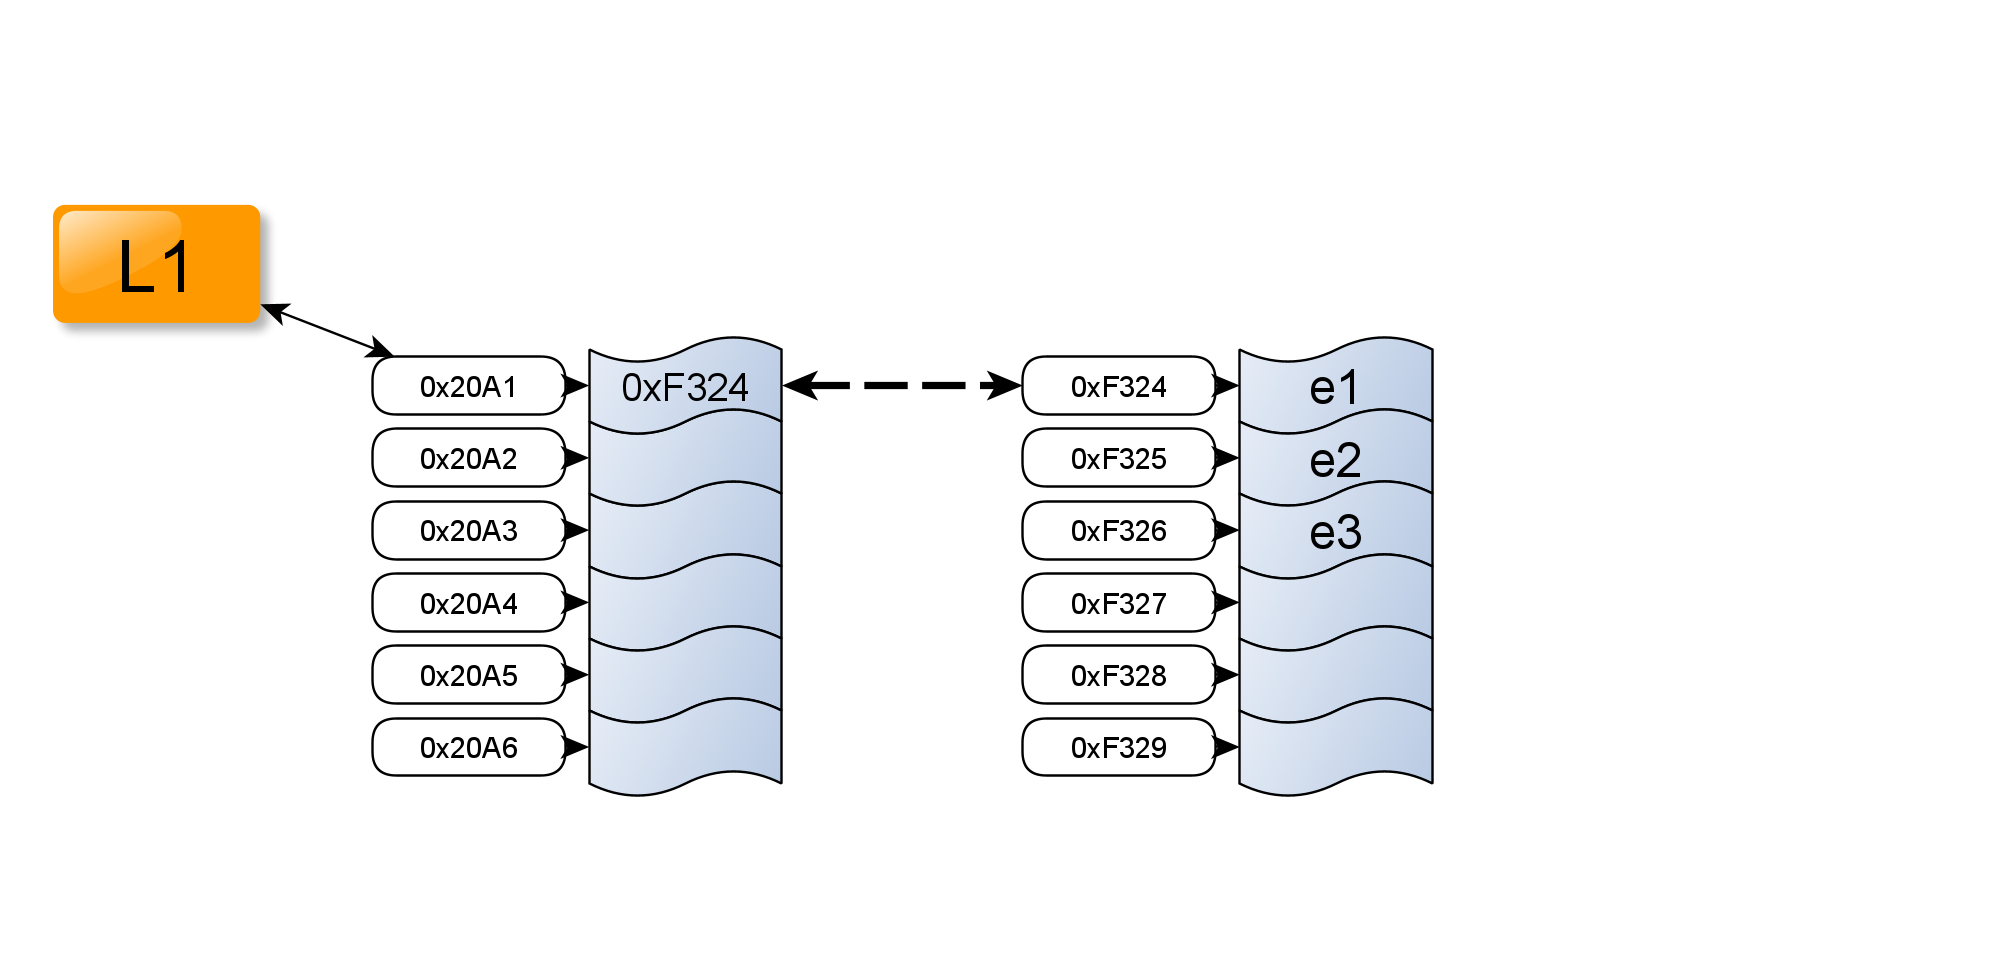
\includegraphics[width=10cm]{img/L2}\\ L1 contient \alert{l'adresse du début de la plage mémoire}.}
	\only<5>{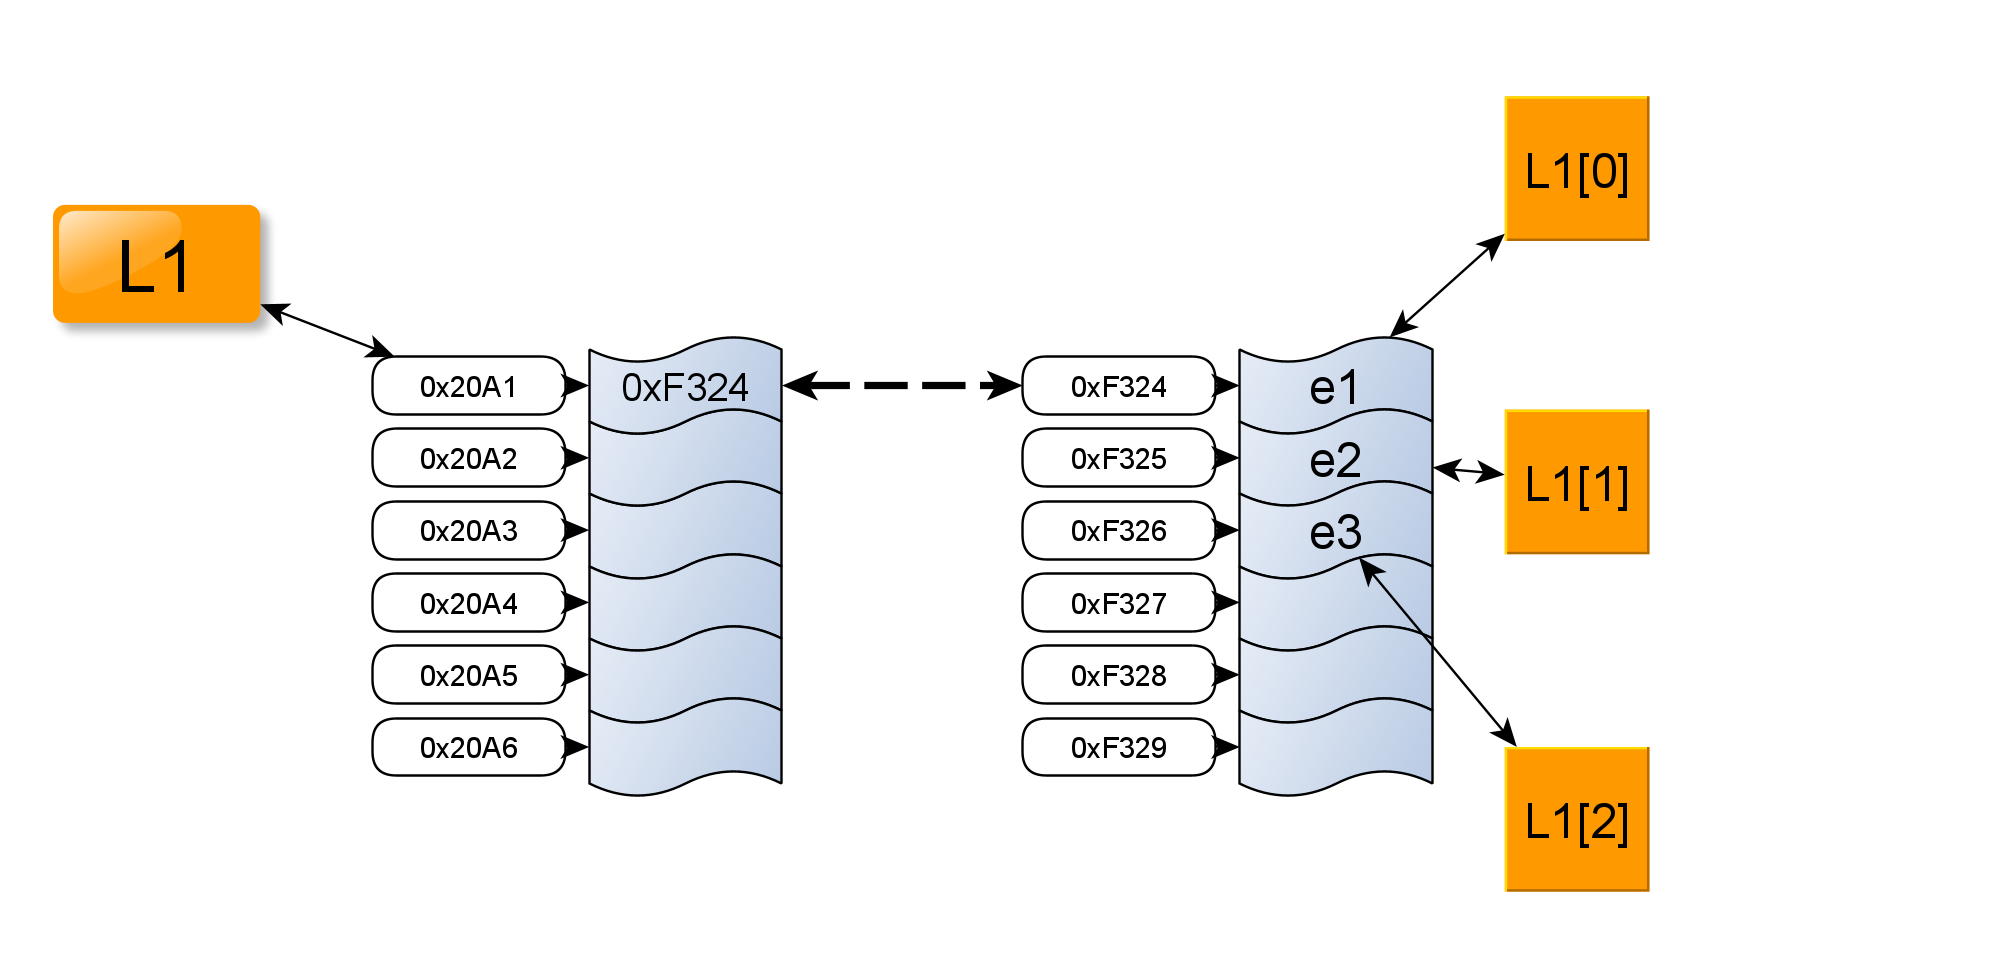
\includegraphics[width=10cm]{img/L3}\\ }
	\only<6>{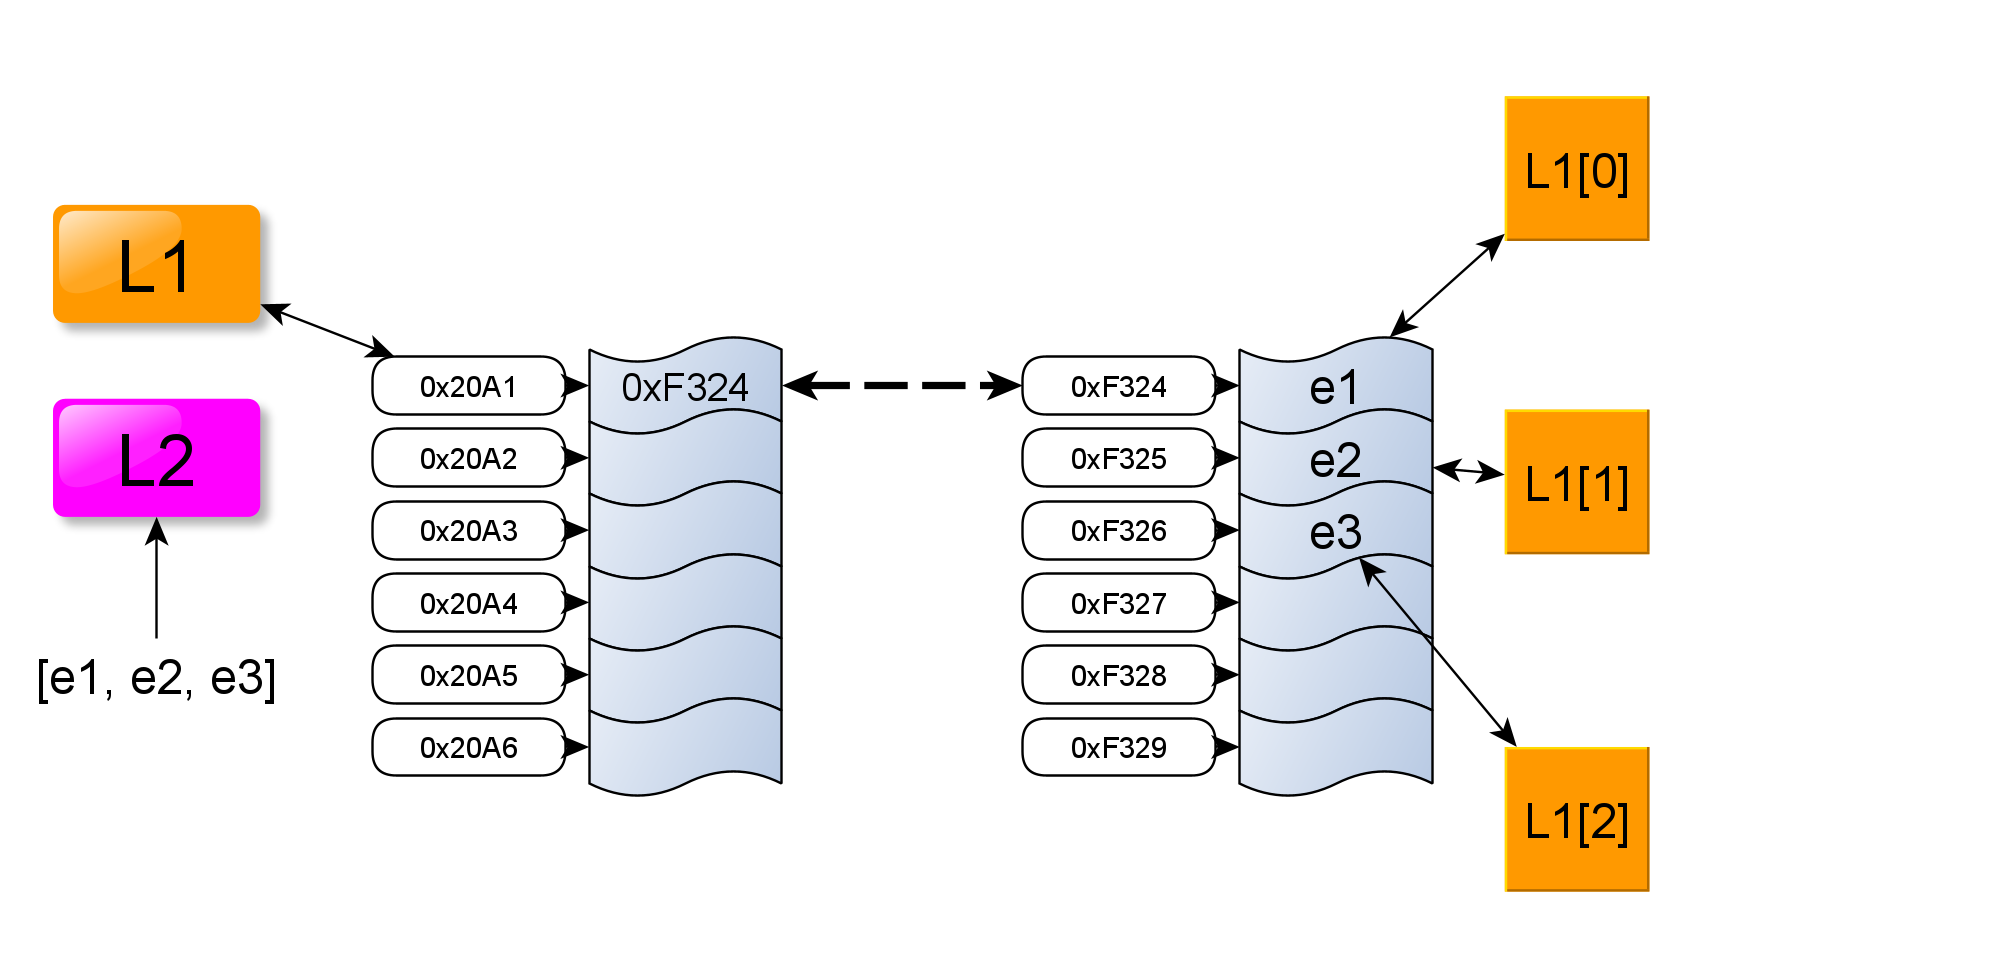
\includegraphics[width=10cm]{img/L4}\\ On affecte [e1, e2, e3] à L2.}
	\only<7>{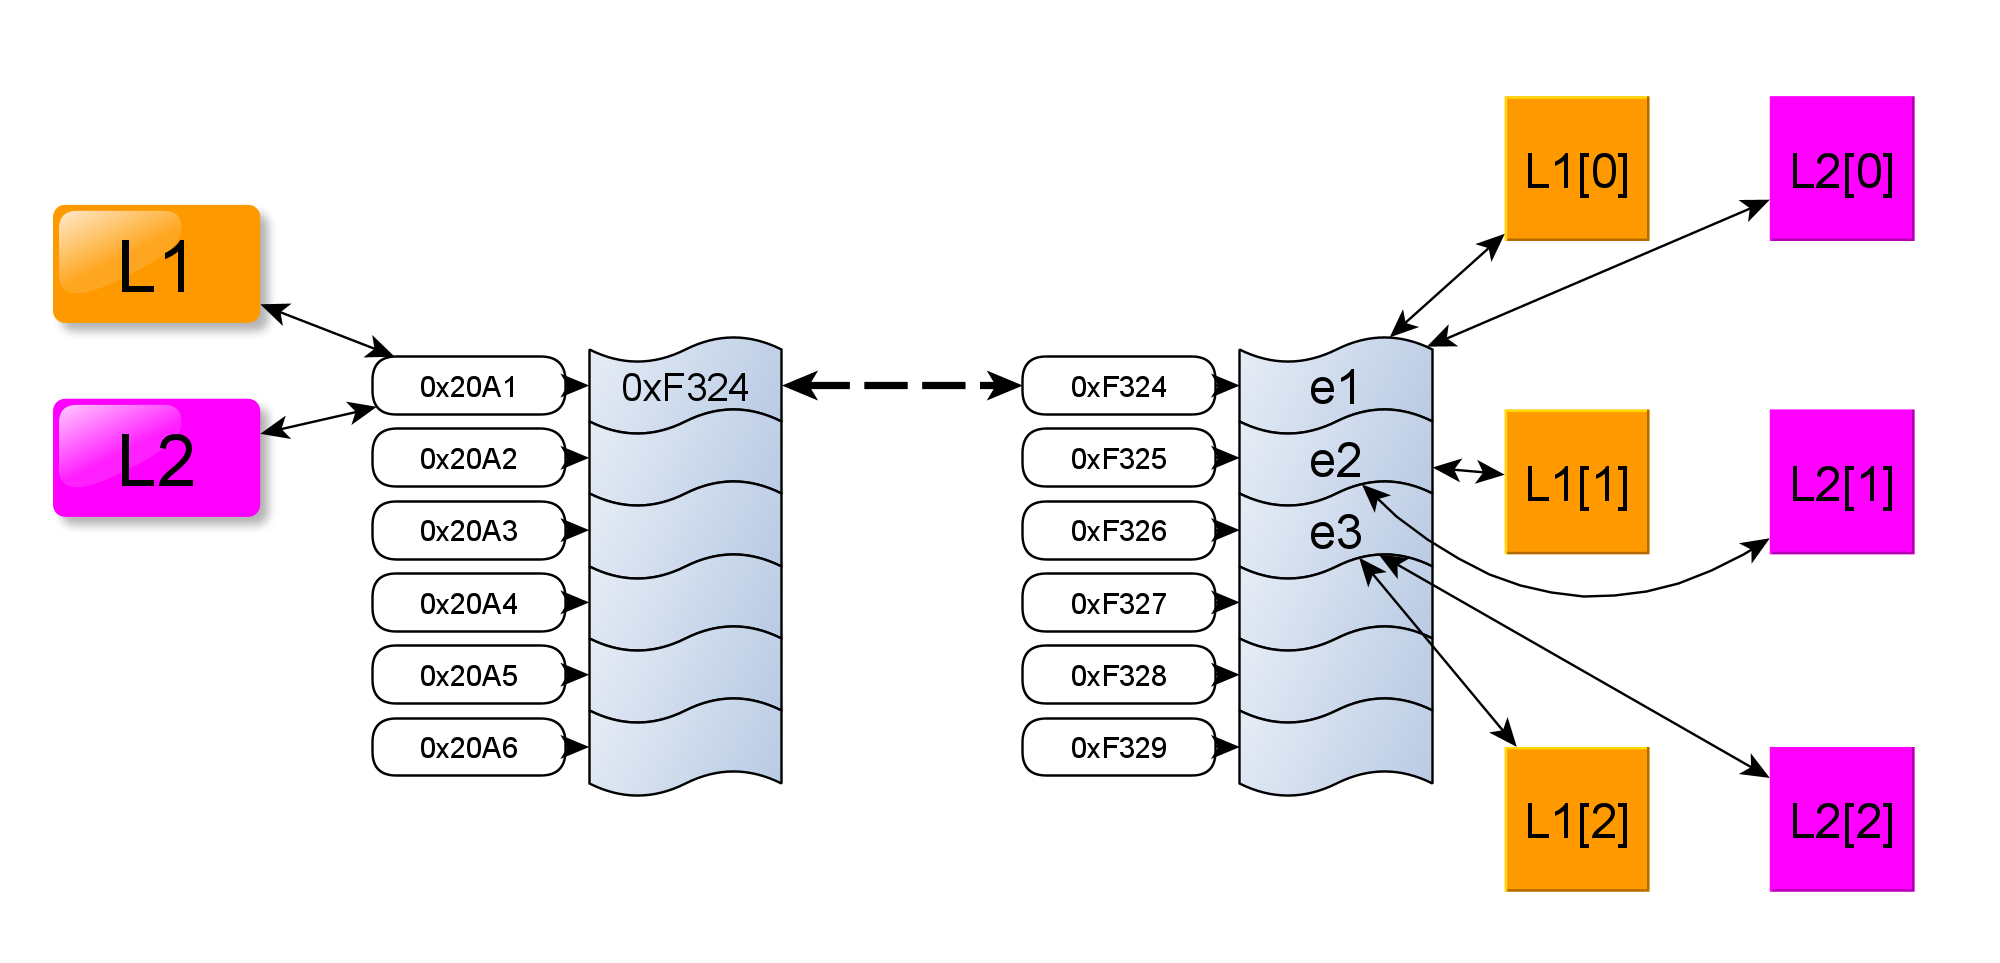
\includegraphics[width=10cm]{img/L5}\\ L2 contient la même adresse que A.}
	\only<8>{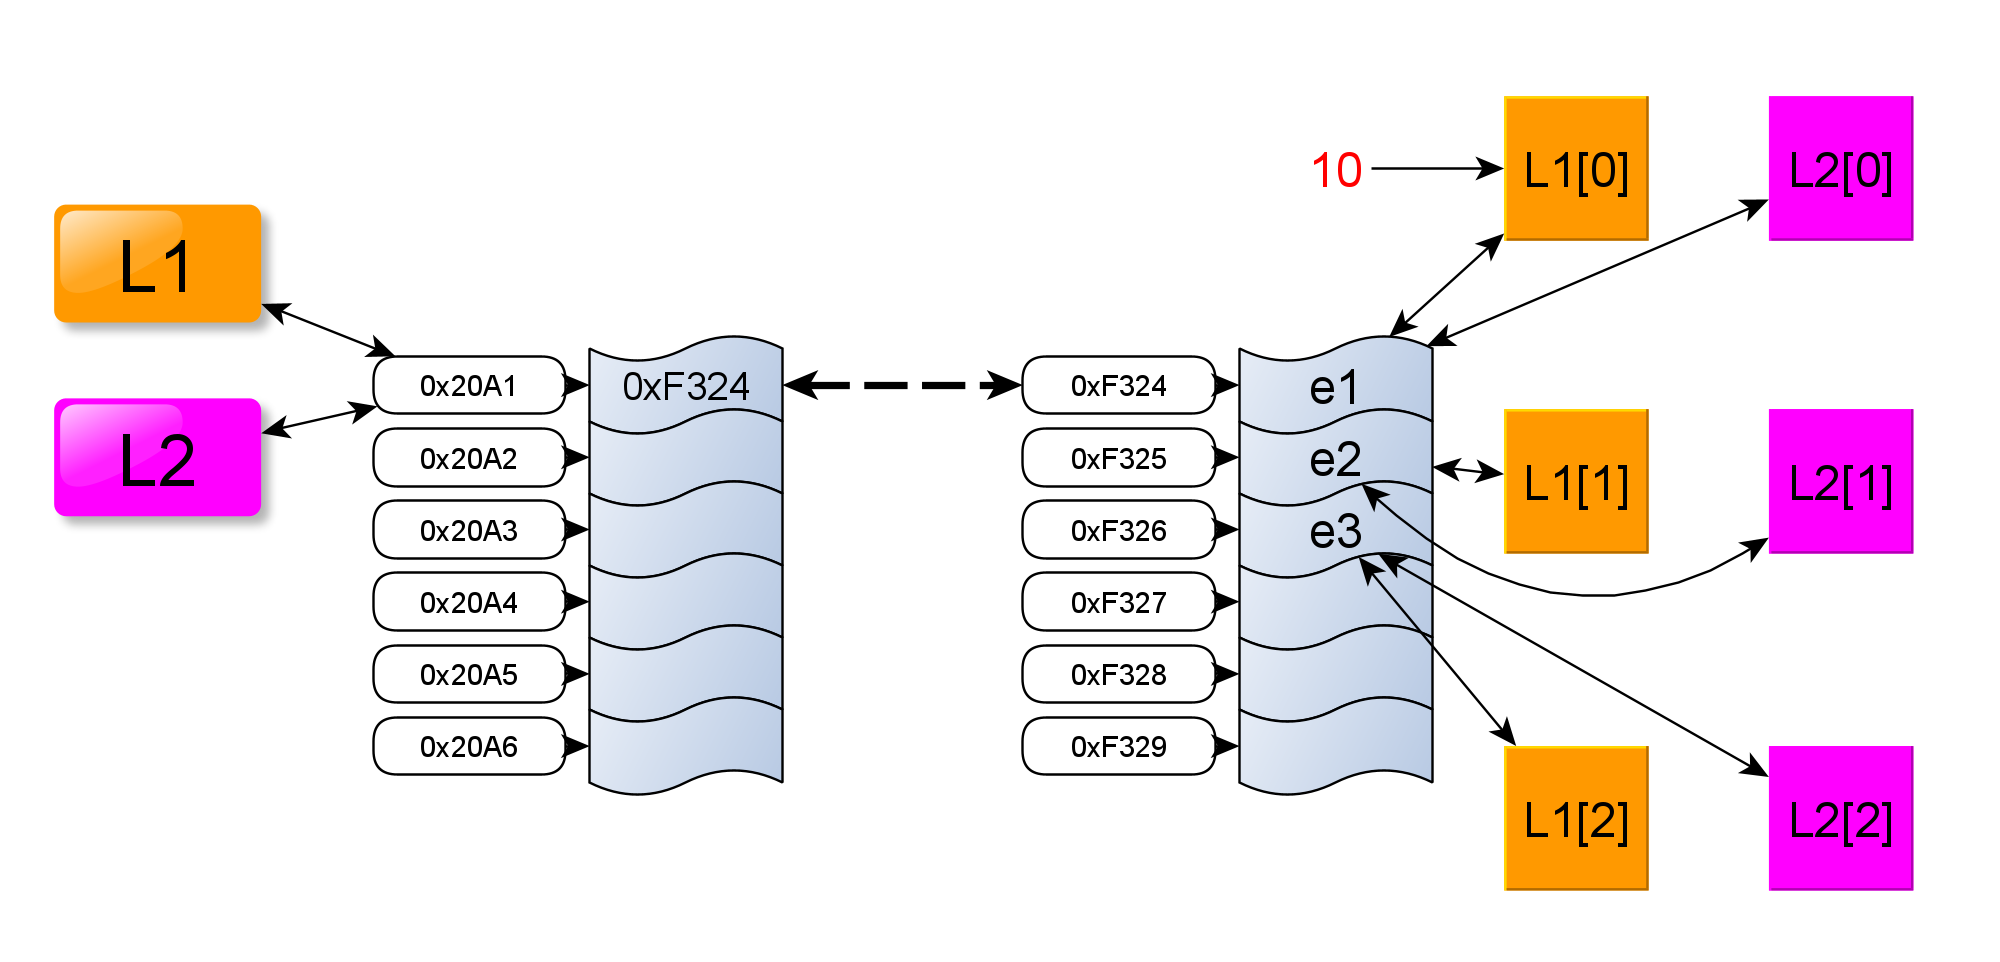
\includegraphics[width=10cm]{img/L6}\\ Si on affecte 10 à L1[0]}
	\only<9>{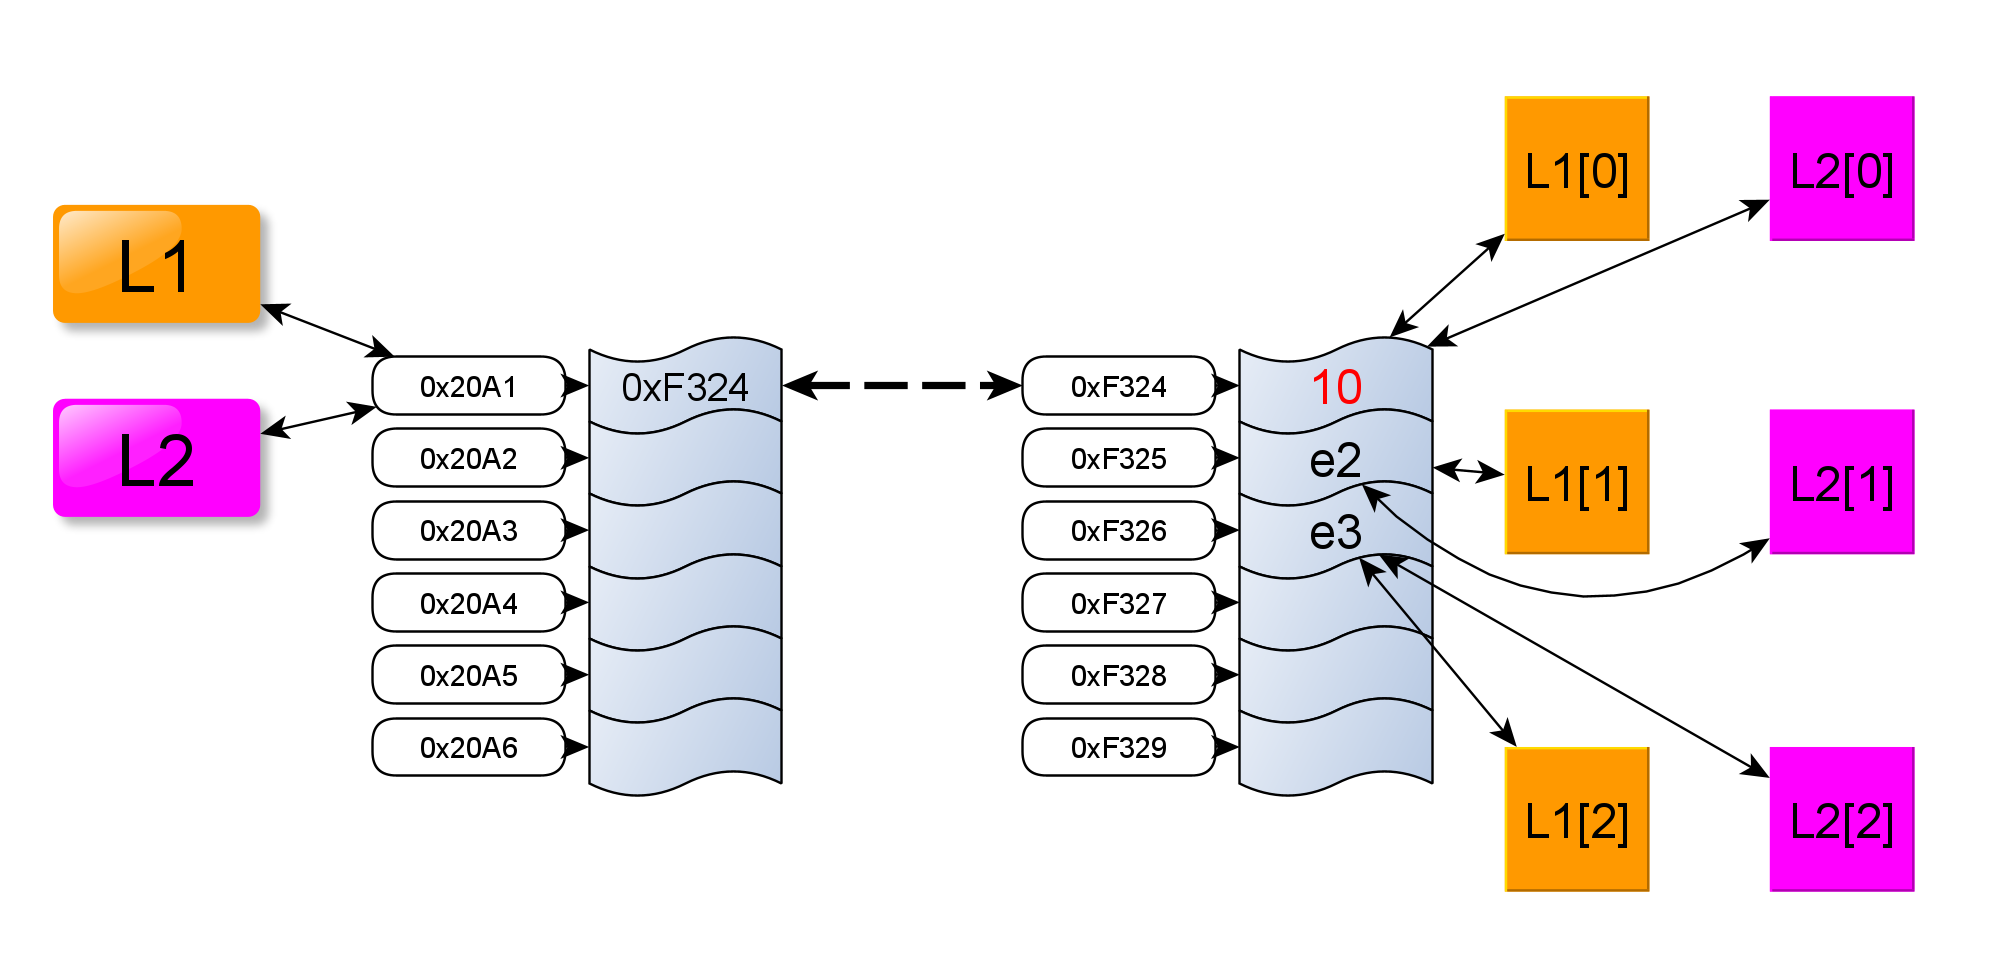
\includegraphics[width=10cm]{img/L7}\\ Alors L2[0] vaut 10 également.}
\end{frame}

\section{Parcourir une liste}
\begin{frame}[fragile]{Parcours selon les indices}\pause
\begin{minted}{python}
L = [54, 65, 123]
n = len(L)
for i in range(n):
    print(L[i])
\end{minted}

\end{frame}

\begin{frame}[fragile]{Parcours selon les valeurs}\pause
\begin{minted}{python}
L = [54, 65, 123]
for x in L:
    print(x)
\end{minted}

\end{frame}

\end{document}